\documentclass[]{article}
\usepackage{lmodern}
\usepackage{amssymb,amsmath}
\usepackage{ifxetex,ifluatex}
\usepackage{fixltx2e} % provides \textsubscript
\ifnum 0\ifxetex 1\fi\ifluatex 1\fi=0 % if pdftex
  \usepackage[T1]{fontenc}
  \usepackage[utf8]{inputenc}
\else % if luatex or xelatex
  \ifxetex
    \usepackage{mathspec}
  \else
    \usepackage{fontspec}
  \fi
  \defaultfontfeatures{Ligatures=TeX,Scale=MatchLowercase}
\fi
% use upquote if available, for straight quotes in verbatim environments
\IfFileExists{upquote.sty}{\usepackage{upquote}}{}
% use microtype if available
\IfFileExists{microtype.sty}{%
\usepackage[]{microtype}
\UseMicrotypeSet[protrusion]{basicmath} % disable protrusion for tt fonts
}{}
\PassOptionsToPackage{hyphens}{url} % url is loaded by hyperref
\usepackage[unicode=true]{hyperref}
\hypersetup{
            pdftitle={Survey32 Writeup},
            pdfborder={0 0 0},
            breaklinks=true}
\urlstyle{same}  % don't use monospace font for urls
\usepackage[margin=1in]{geometry}
\usepackage{graphicx,grffile}
\makeatletter
\def\maxwidth{\ifdim\Gin@nat@width>\linewidth\linewidth\else\Gin@nat@width\fi}
\def\maxheight{\ifdim\Gin@nat@height>\textheight\textheight\else\Gin@nat@height\fi}
\makeatother
% Scale images if necessary, so that they will not overflow the page
% margins by default, and it is still possible to overwrite the defaults
% using explicit options in \includegraphics[width, height, ...]{}
\setkeys{Gin}{width=\maxwidth,height=\maxheight,keepaspectratio}
\IfFileExists{parskip.sty}{%
\usepackage{parskip}
}{% else
\setlength{\parindent}{0pt}
\setlength{\parskip}{6pt plus 2pt minus 1pt}
}
\setlength{\emergencystretch}{3em}  % prevent overfull lines
\providecommand{\tightlist}{%
  \setlength{\itemsep}{0pt}\setlength{\parskip}{0pt}}
\setcounter{secnumdepth}{0}
% Redefines (sub)paragraphs to behave more like sections
\ifx\paragraph\undefined\else
\let\oldparagraph\paragraph
\renewcommand{\paragraph}[1]{\oldparagraph{#1}\mbox{}}
\fi
\ifx\subparagraph\undefined\else
\let\oldsubparagraph\subparagraph
\renewcommand{\subparagraph}[1]{\oldsubparagraph{#1}\mbox{}}
\fi

% set default figure placement to htbp
\makeatletter
\def\fps@figure{htbp}
\makeatother


\title{Survey32 Writeup}
\author{}
\date{\vspace{-2.5em}}

\begin{document}
\maketitle

\subsection{Who Are the Soldiers?}\label{who-are-the-soldiers}

Survey 32 was given out to soldiers in 1943, approximately 5 years
before the military was integrated. The survey was passed out to 7442
black soldiers and 4793 white soldiers and asked for basic demographic
information, career aspirations, and more but of interests to us, Survey
32 asked the soldiers for their opinions on integration of military
outfits. Our questions of interest are regarding age, education,
enlistment, state, community type, and of course their opinions on
outfits. On the survey these questions were asked in Questions
1,2,3,13,14, and 77 (63 for white soldiers), respectively.

\begin{verbatim}
##      age                    edu      enlist        outfits        state
## 1  21-24 SOME HIGH/TRADE SCHOOL VOLUNTEERED Doesn't Matter         OHIO
## 2  21-24 SOME HIGH/TRADE SCHOOL     DRAFTED      Seperated     ILLINOIS
## 3  21-24              8TH GRADE     DRAFTED      Seperated     ILLINOIS
## 4   <=19              4TH GRADE VOLUNTEERED      Undecided     ILLINOIS
## 5  21-24            HIGH SCHOOL     DRAFTED      Seperated         UTAH
## 6  21-24              8TH GRADE     DRAFTED      Undecided     MISSOURI
## 7     20              4TH GRADE VOLUNTEERED Doesn't Matter PENNSYLVANIA
## 8  21-24            HIGH SCHOOL VOLUNTEERED      Seperated    WISCONSIN
## 9     20              4TH GRADE VOLUNTEERED       Together         OHIO
## 10    20            < 4TH GRADE VOLUNTEERED      Seperated      FLORIDA
##     community  race
## 1  Large City White
## 2  Large City White
## 3  Small Town White
## 4  Large City Black
## 5  Small Town White
## 6        Farm White
## 7        City Black
## 8  Large City White
## 9        City Black
## 10       Town Black
\end{verbatim}

\subsubsection{How Old Are the Soldiers}\label{how-old-are-the-soldiers}

Age was not collected on a continuous scale and was discretized into a
few different age groups. We see that the overwhelming bulk of black
soldiers who were survied were 20 years old with a small portion who
were 19 or younger. In the meanwhile, the white soldiers had more spread
to their ages with most soldiers being between the ages of 21 and 24.

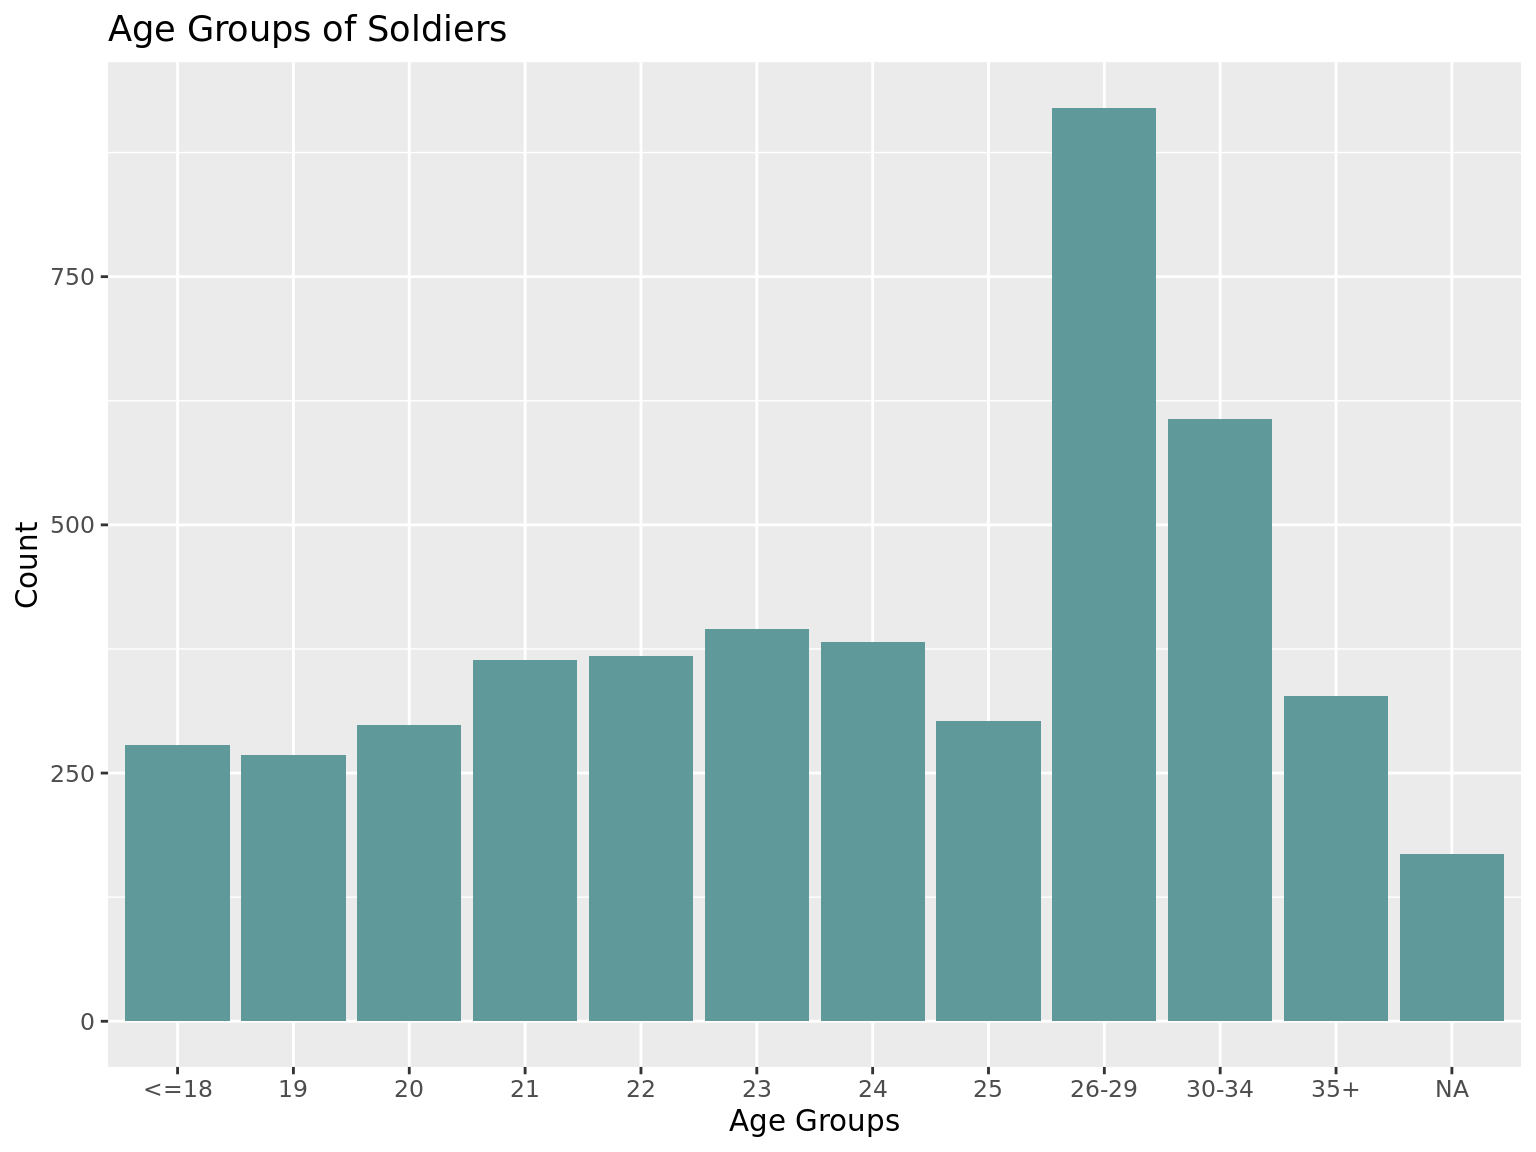
\includegraphics{consildated_overview_files/figure-latex/age-1.pdf}
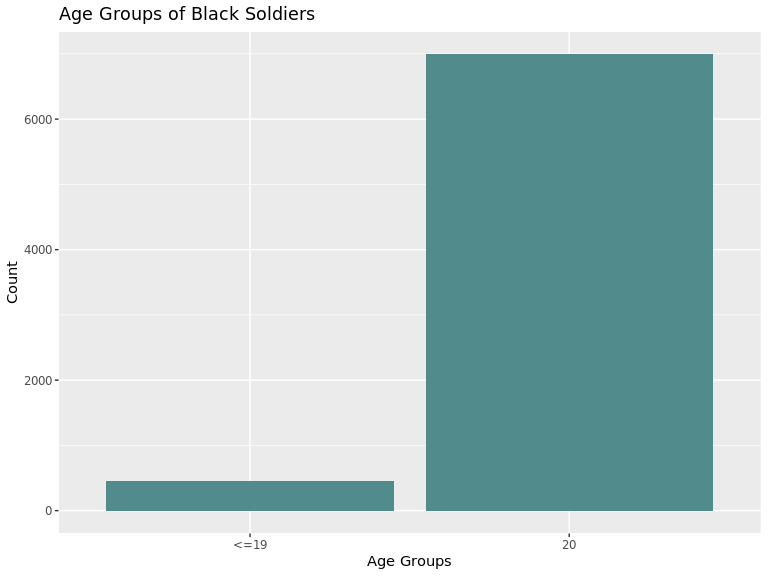
\includegraphics{consildated_overview_files/figure-latex/age-2.pdf}
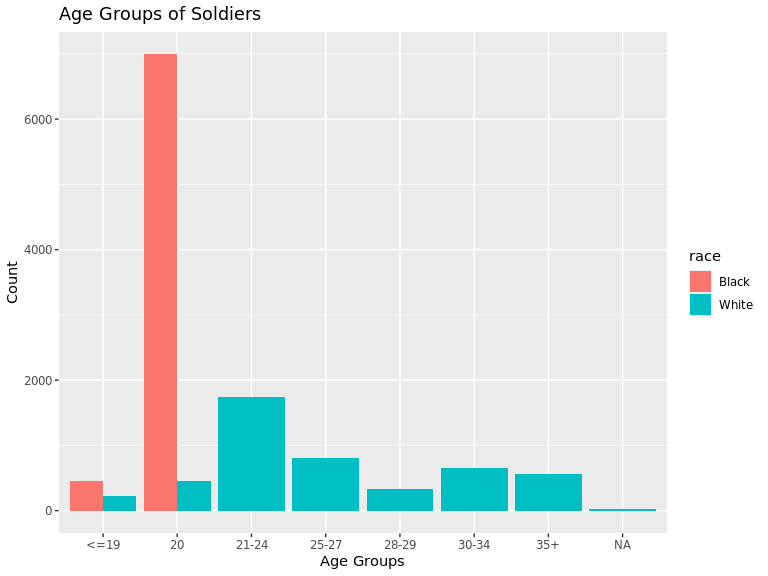
\includegraphics{consildated_overview_files/figure-latex/age-3.pdf}

\begin{verbatim}
## Warning in melt(., id.vars = "age"): The melt generic in data.table has been
## passed a data.frame and will attempt to redirect to the relevant reshape2
## method; please note that reshape2 is deprecated, and this redirection is now
## deprecated as well. To continue using melt methods from reshape2 while both
## libraries are attached, e.g. melt.list, you can prepend the namespace like
## reshape2::melt(.). In the next version, this warning will become an error.
\end{verbatim}

\begin{verbatim}
## Warning: Removed 6 rows containing missing values (geom_bar).
\end{verbatim}

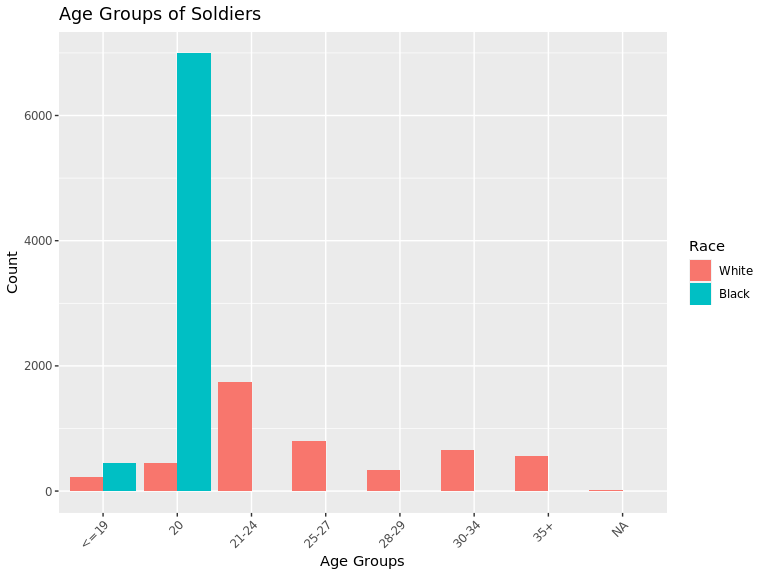
\includegraphics{consildated_overview_files/figure-latex/age-4.pdf}

\subsubsection{How Far in School Were
They?}\label{how-far-in-school-were-they}

If we look at education now we see that again black soldiers have littel
spread in their education. Remarkably, all of the black soldiers survied
have less than a 5th grade education at the time. Meanwhile, the bulk of
the white soldiers have had a high school/some high school.

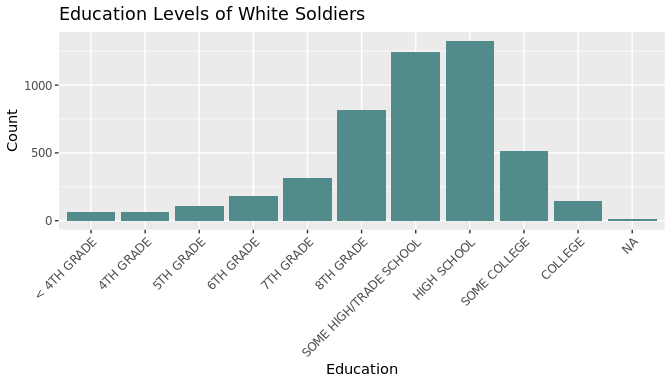
\includegraphics{consildated_overview_files/figure-latex/edu-1.pdf}
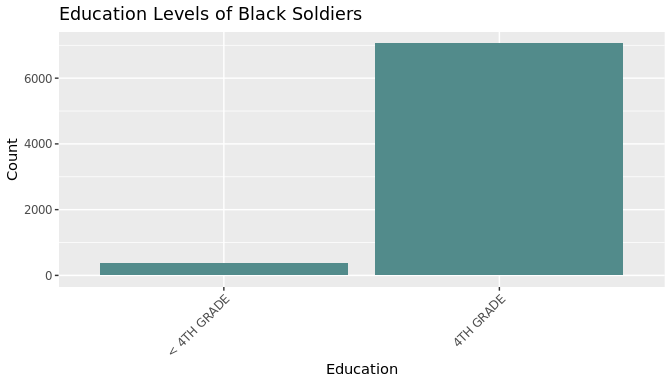
\includegraphics{consildated_overview_files/figure-latex/edu-2.pdf}

\begin{verbatim}
## Warning in melt(., id.vars = "edu"): The melt generic in data.table has been
## passed a data.frame and will attempt to redirect to the relevant reshape2
## method; please note that reshape2 is deprecated, and this redirection is now
## deprecated as well. To continue using melt methods from reshape2 while both
## libraries are attached, e.g. melt.list, you can prepend the namespace like
## reshape2::melt(.). In the next version, this warning will become an error.
\end{verbatim}

\begin{verbatim}
## Warning: Removed 9 rows containing missing values (geom_bar).
\end{verbatim}

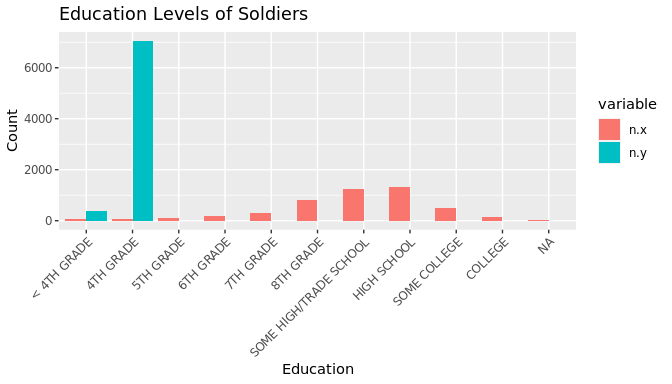
\includegraphics{consildated_overview_files/figure-latex/edu-3.pdf}
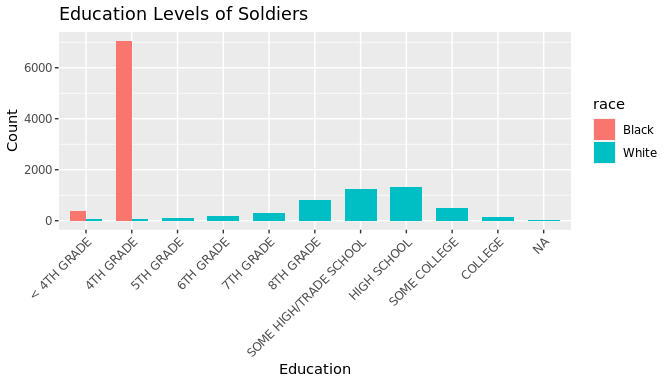
\includegraphics{consildated_overview_files/figure-latex/edu-4.pdf}

\begin{verbatim}
## Warning in melt(., id.vars = "edu"): The melt generic in data.table has been
## passed a data.frame and will attempt to redirect to the relevant reshape2
## method; please note that reshape2 is deprecated, and this redirection is now
## deprecated as well. To continue using melt methods from reshape2 while both
## libraries are attached, e.g. melt.list, you can prepend the namespace like
## reshape2::melt(.). In the next version, this warning will become an error.

## Warning in melt(., id.vars = "edu"): Removed 9 rows containing missing values
## (geom_bar).
\end{verbatim}

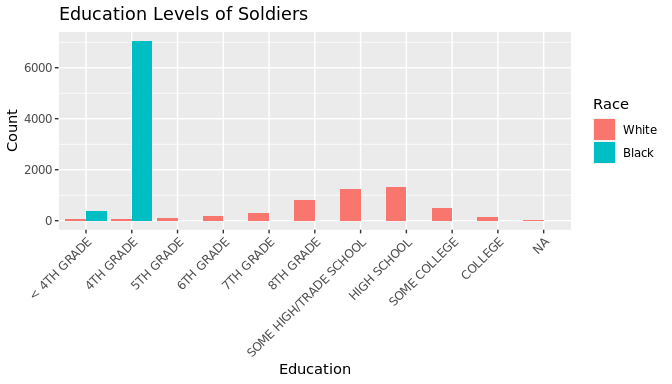
\includegraphics{consildated_overview_files/figure-latex/edu-5.pdf}

\begin{verbatim}
## Warning in melt(., id.vars = "edu"): The melt generic in data.table has been
## passed a data.frame and will attempt to redirect to the relevant reshape2
## method; please note that reshape2 is deprecated, and this redirection is now
## deprecated as well. To continue using melt methods from reshape2 while both
## libraries are attached, e.g. melt.list, you can prepend the namespace like
## reshape2::melt(.). In the next version, this warning will become an error.

## Warning in melt(., id.vars = "edu"): Removed 9 rows containing missing values
## (geom_bar).
\end{verbatim}

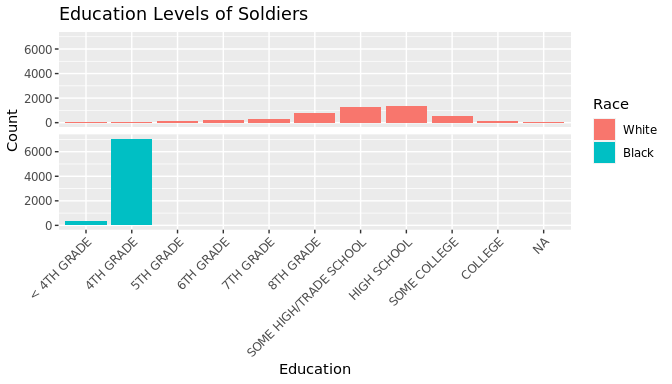
\includegraphics{consildated_overview_files/figure-latex/edu-6.pdf}

\subsubsection{How Did They End Up in the
Military}\label{how-did-they-end-up-in-the-military}

Something interesting arises here were we find that vast majority of the
black soldiers actually volunteered to join the military whereas about
3/4 of the survied white soldiers were drafted and the remaining
soldiers were moslty volunteers and a few were from the National Guard.
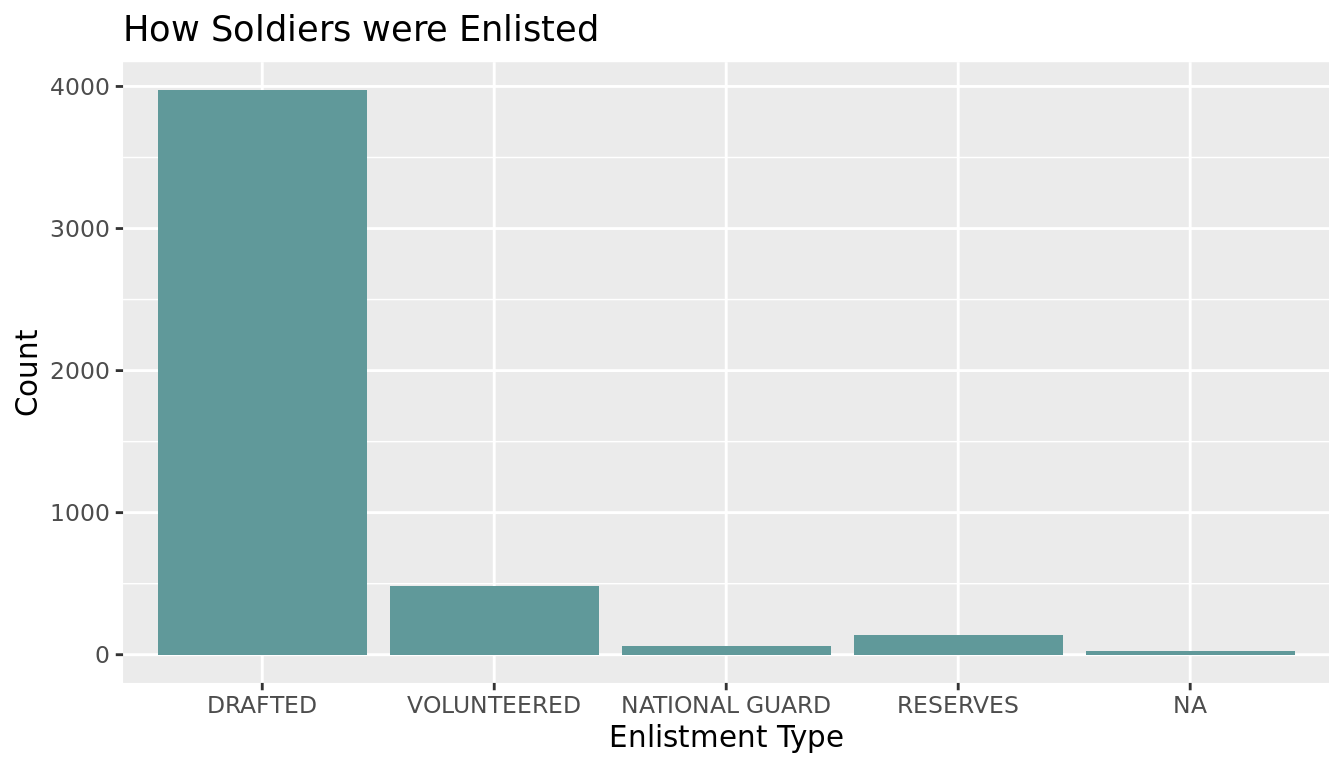
\includegraphics{consildated_overview_files/figure-latex/enlist-1.pdf}
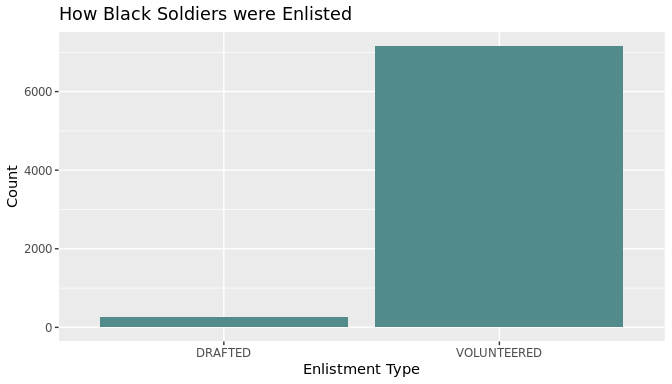
\includegraphics{consildated_overview_files/figure-latex/enlist-2.pdf}

\begin{verbatim}
## Warning in melt(., id.vars = "enlist"): The melt generic in data.table has
## been passed a data.frame and will attempt to redirect to the relevant reshape2
## method; please note that reshape2 is deprecated, and this redirection is now
## deprecated as well. To continue using melt methods from reshape2 while both
## libraries are attached, e.g. melt.list, you can prepend the namespace like
## reshape2::melt(.). In the next version, this warning will become an error.
\end{verbatim}

\begin{verbatim}
## Warning: Removed 2 rows containing missing values (geom_bar).
\end{verbatim}

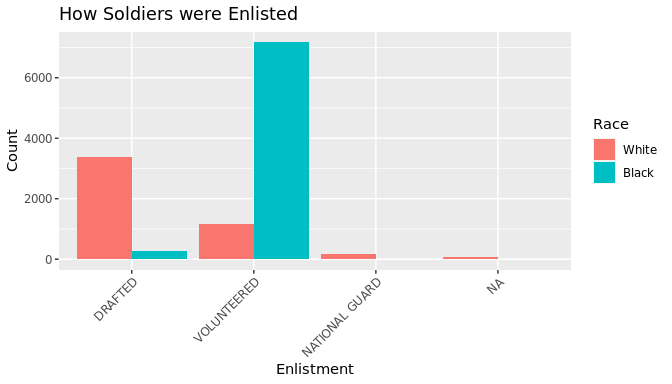
\includegraphics{consildated_overview_files/figure-latex/enlist-3.pdf}

\subsubsection{Where Are the Soldiers
From?}\label{where-are-the-soldiers-from}

Expectedly, most of the soldiers hailed from the most populous states at
the time. White soldiers were mostly from Illionois, Pennsylvania, Ney
York, Texas, and Michigan while black soldiers were mostly from Texas,
New York, Illinois, Pennsylvania, and Ohio. Note that the top 4 states
for white soldiers had similar amounts of soldiers but there was a sever
drop off in representation of black soldiers from other states after
Texas and New York.

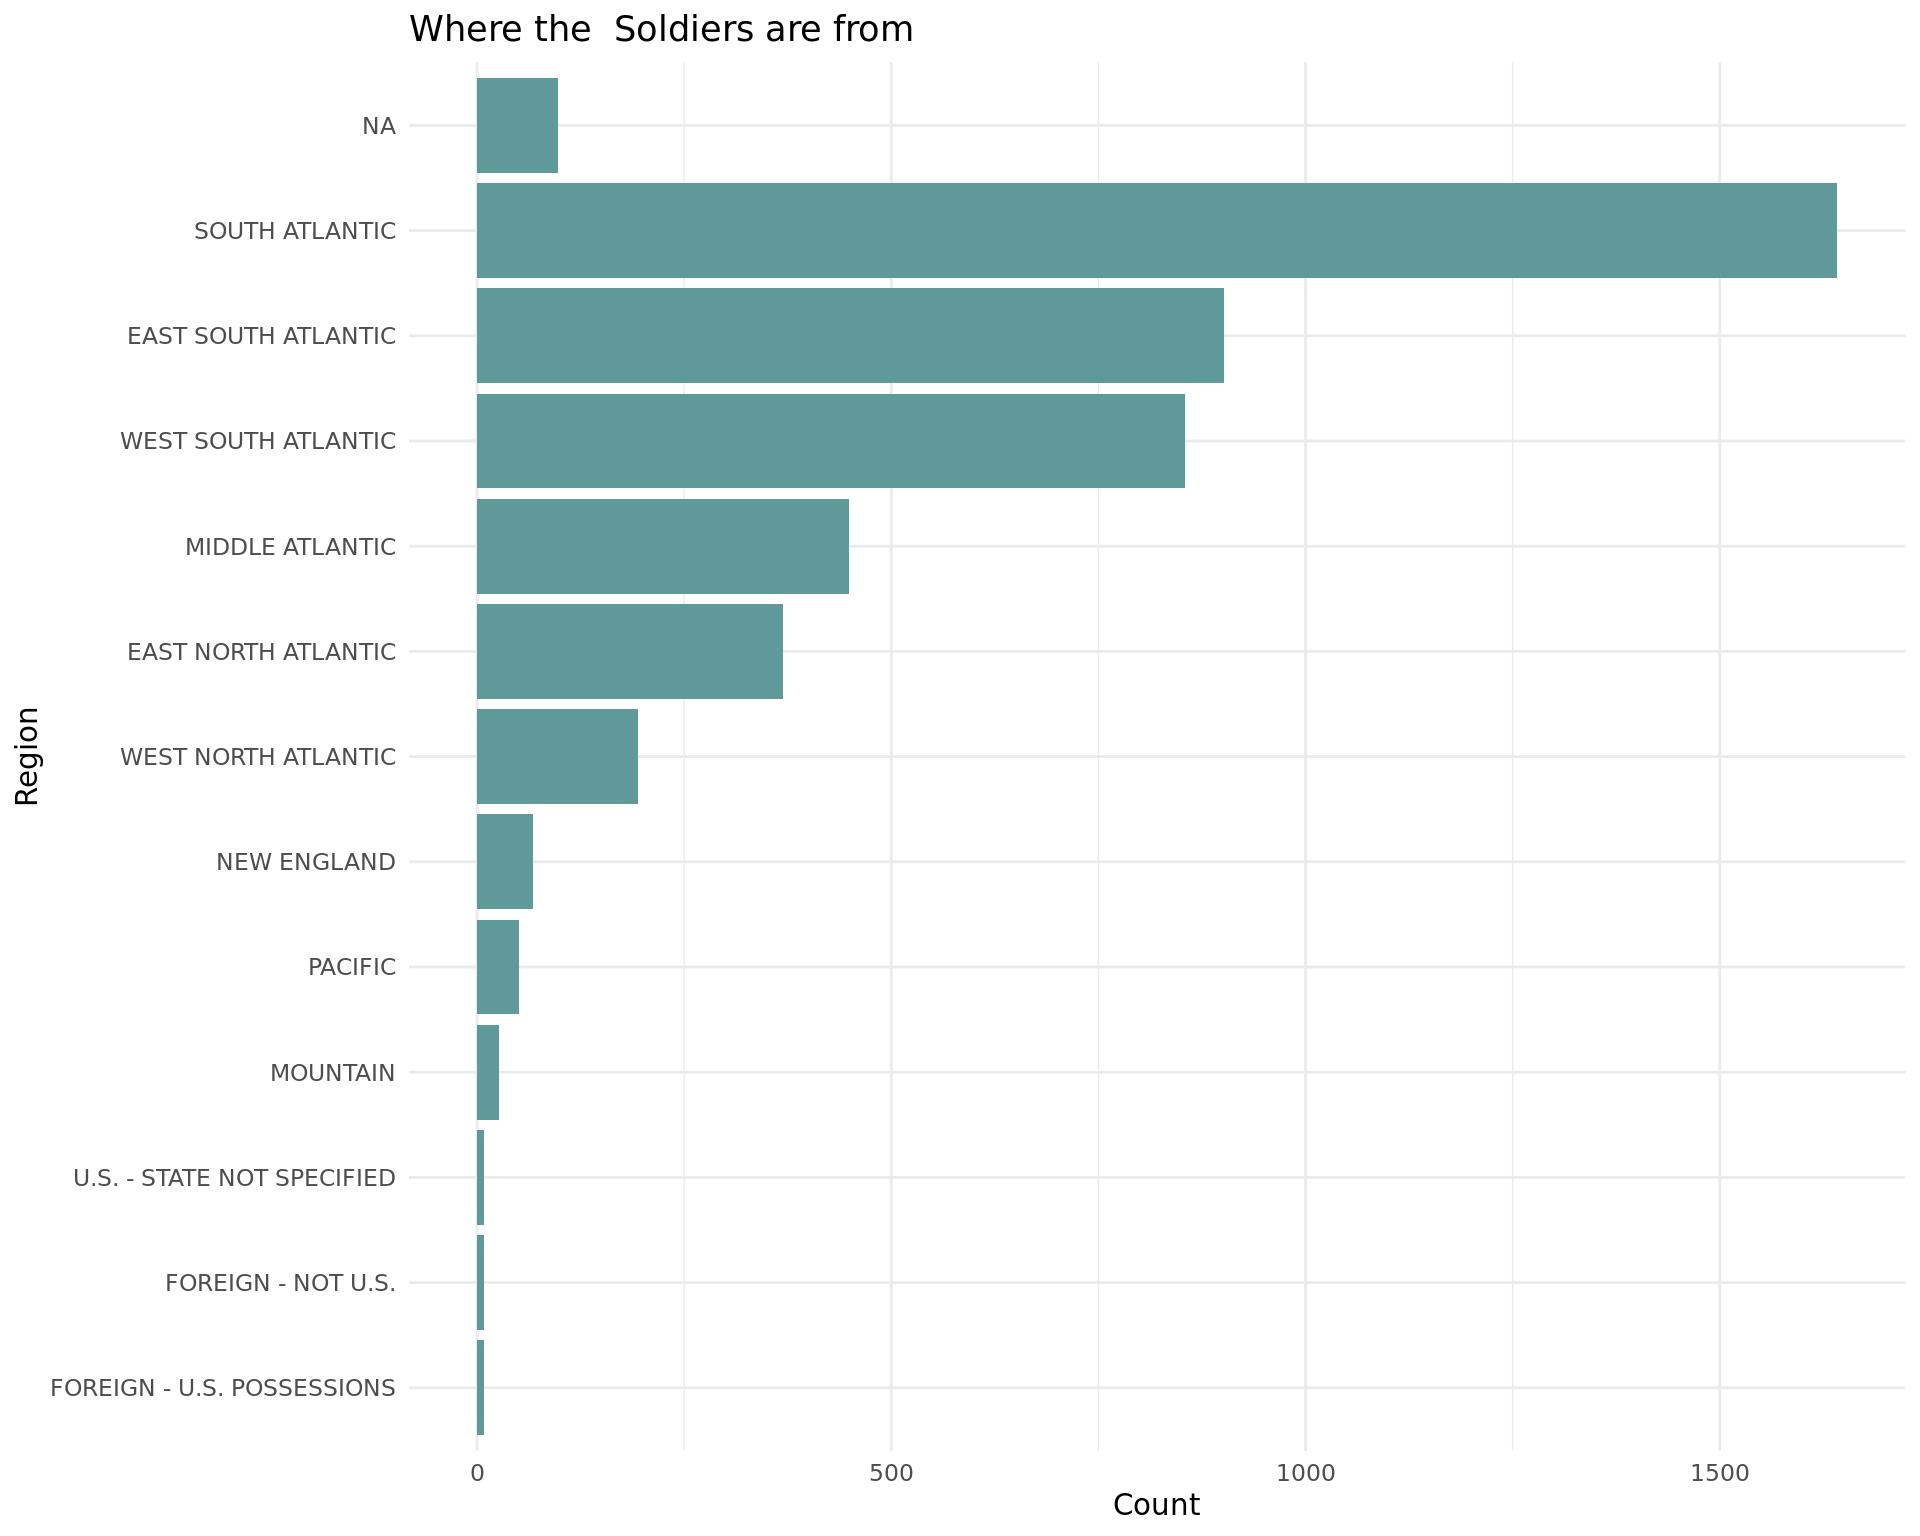
\includegraphics{consildated_overview_files/figure-latex/state-1.pdf}
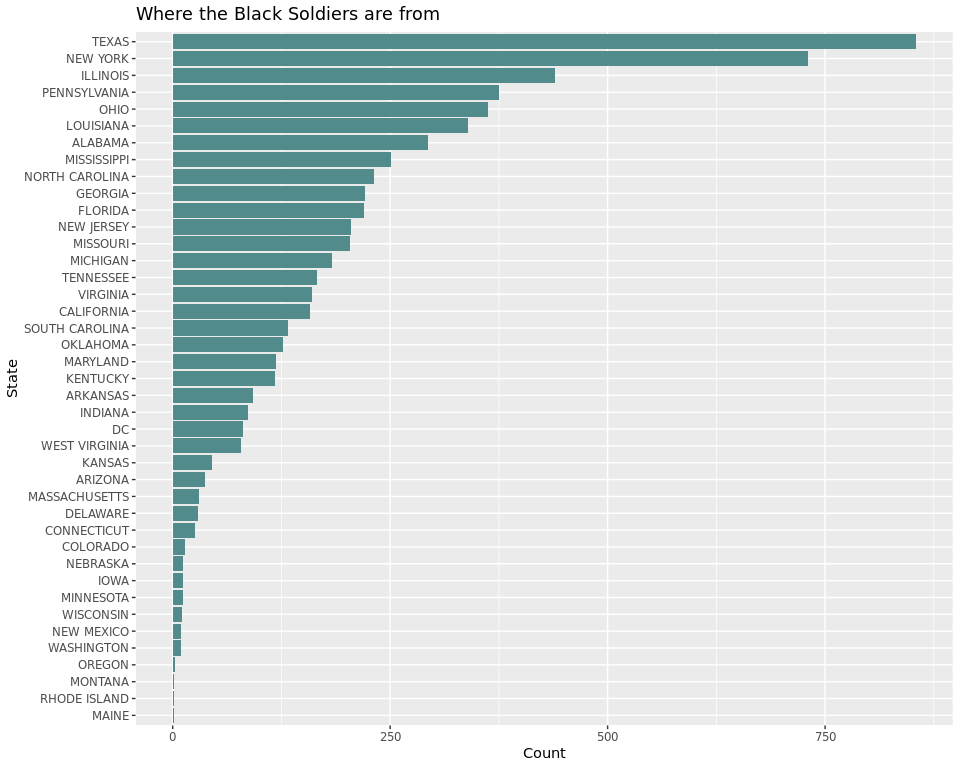
\includegraphics{consildated_overview_files/figure-latex/state-2.pdf}

\begin{verbatim}
## Warning in melt(., id.vars = "state"): The melt generic in data.table has
## been passed a data.frame and will attempt to redirect to the relevant reshape2
## method; please note that reshape2 is deprecated, and this redirection is now
## deprecated as well. To continue using melt methods from reshape2 while both
## libraries are attached, e.g. melt.list, you can prepend the namespace like
## reshape2::melt(.). In the next version, this warning will become an error.
\end{verbatim}

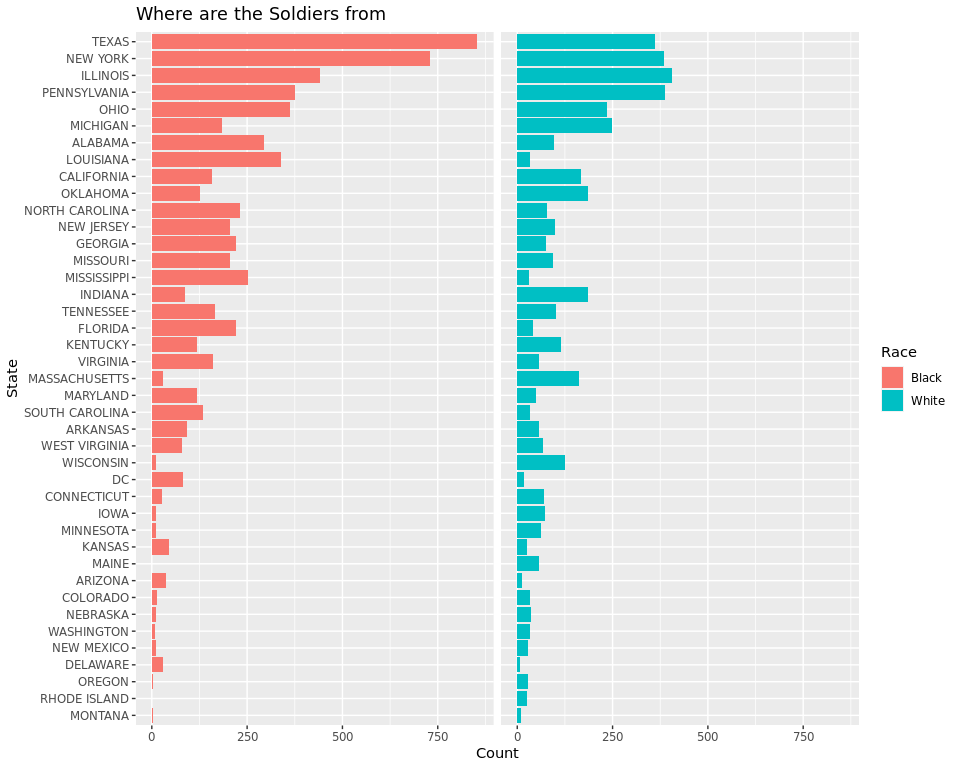
\includegraphics{consildated_overview_files/figure-latex/state-3.pdf}

\begin{verbatim}
## `summarise()` ungrouping output (override with `.groups` argument)
\end{verbatim}

\begin{verbatim}
## Warning: Use of `map_df$x` is discouraged. Use `x` instead.
\end{verbatim}

\begin{verbatim}
## Warning: Use of `map_df$y` is discouraged. Use `y` instead.
\end{verbatim}

\begin{verbatim}
## Warning: Use of `map_df$group` is discouraged. Use `group` instead.
\end{verbatim}

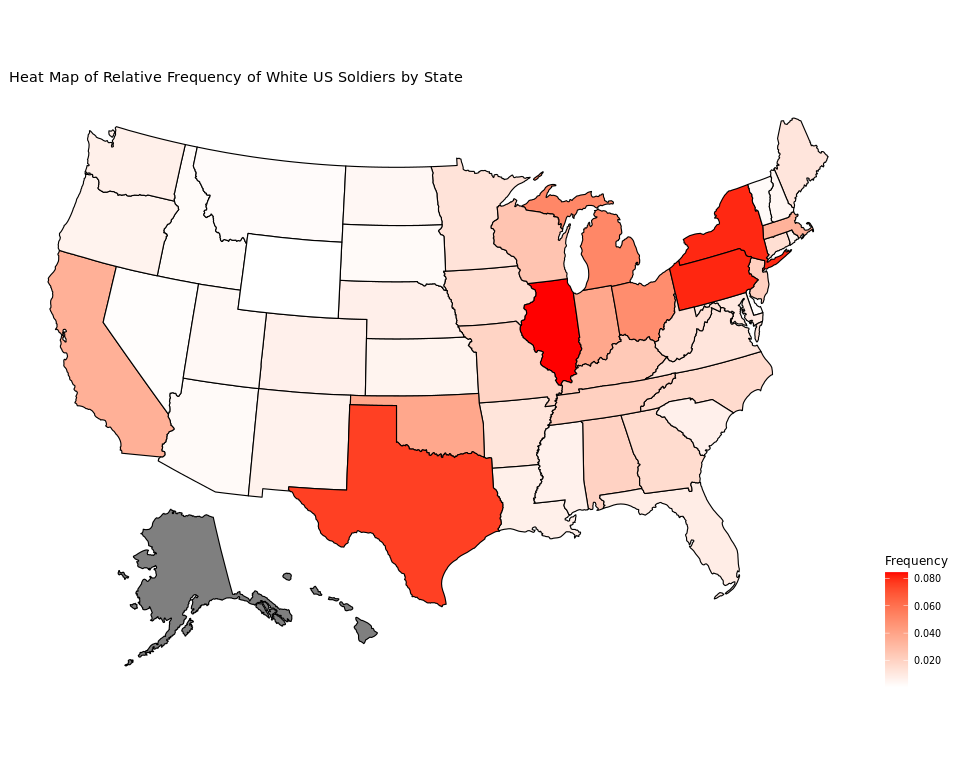
\includegraphics{consildated_overview_files/figure-latex/state-4.pdf}

\begin{verbatim}
## `summarise()` ungrouping output (override with `.groups` argument)
\end{verbatim}

\begin{verbatim}
## Warning: Use of `map_df$x` is discouraged. Use `x` instead.
\end{verbatim}

\begin{verbatim}
## Warning: Use of `map_df$y` is discouraged. Use `y` instead.
\end{verbatim}

\begin{verbatim}
## Warning: Use of `map_df$group` is discouraged. Use `group` instead.
\end{verbatim}

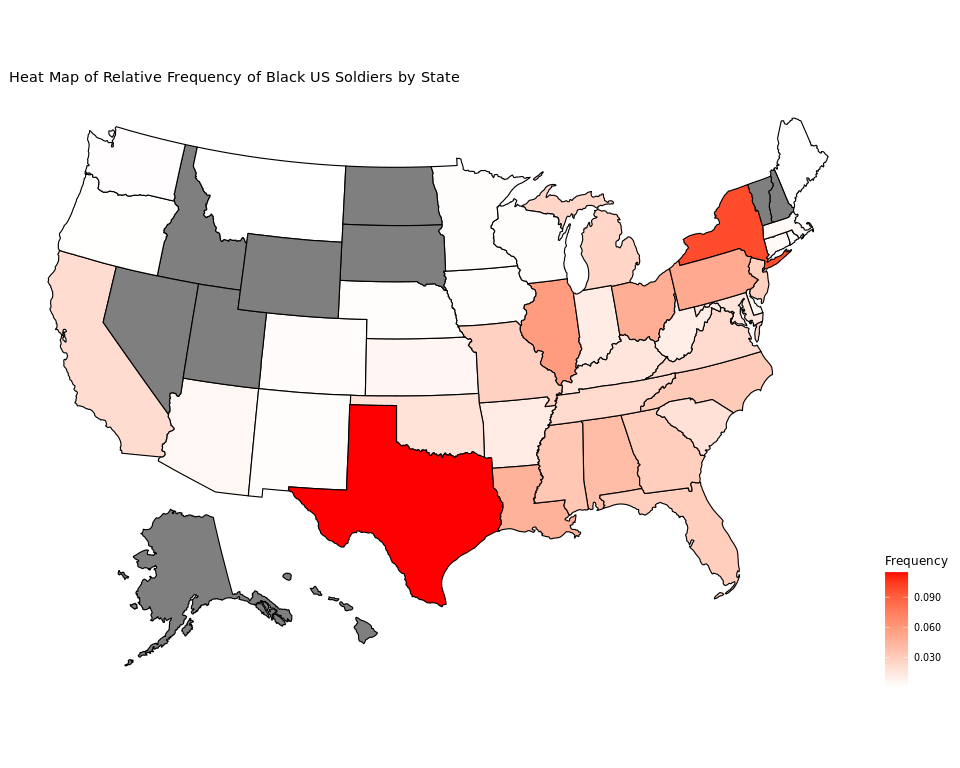
\includegraphics{consildated_overview_files/figure-latex/state-5.pdf}

\subsubsection{What sort of places did they live
in?}\label{what-sort-of-places-did-they-live-in}

As expected, most soldiers whose home communities are large cities had
the most representation across both groups. White soldiers saw roughly
equal representation from soldiers who came from a farm, town, or city
with actually slightly less people from cities. On the otherhand, the
next community with the largest representation for black soldiers was a
city followed by farms and towns which had approximately similar
contributions.

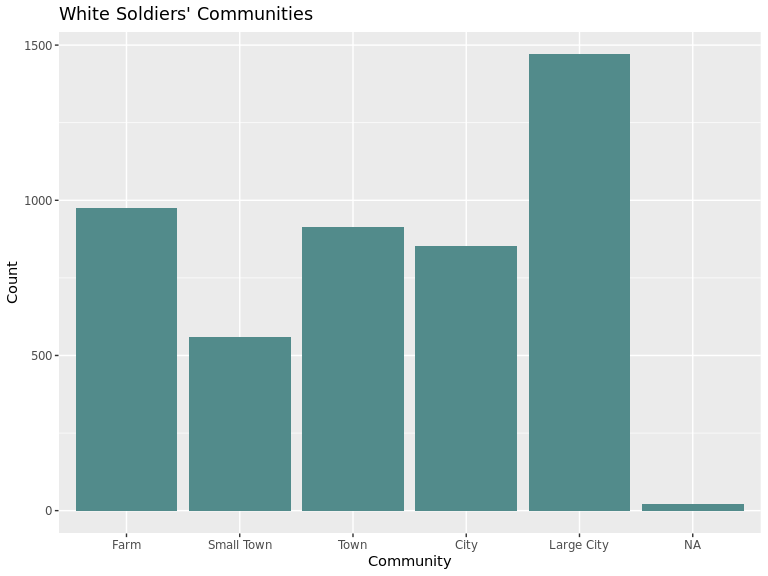
\includegraphics{consildated_overview_files/figure-latex/community-1.pdf}
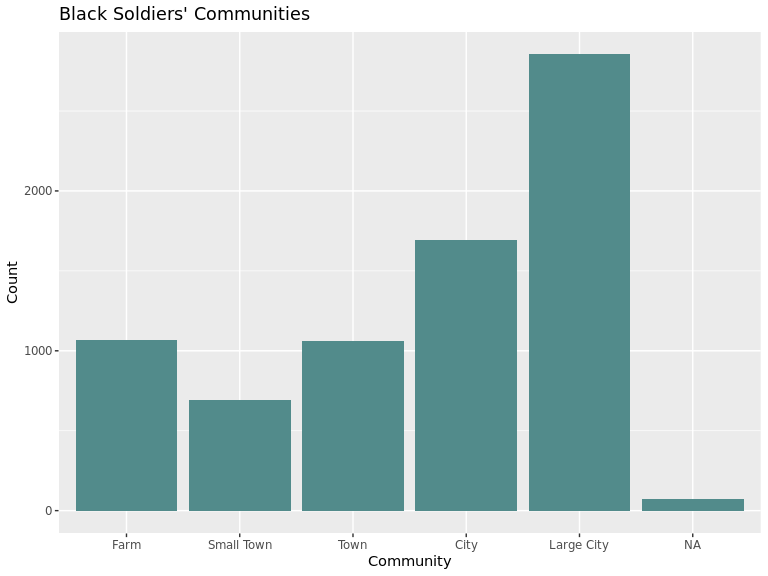
\includegraphics{consildated_overview_files/figure-latex/community-2.pdf}
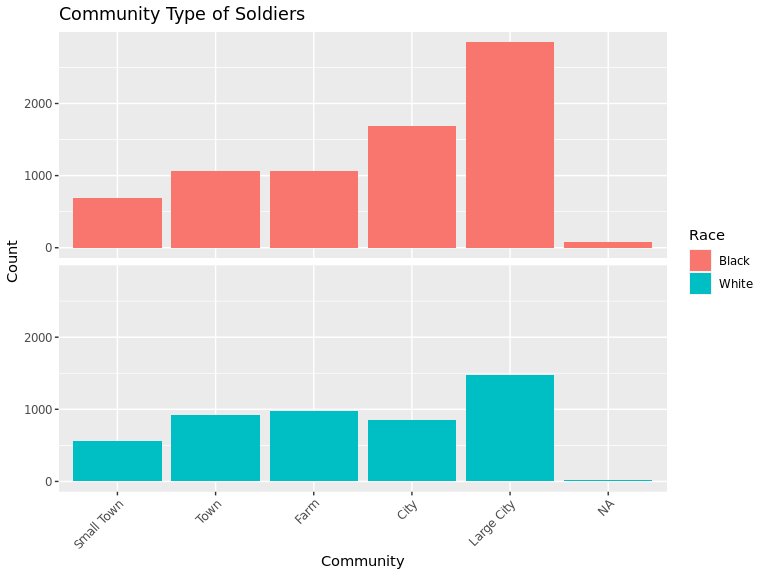
\includegraphics{consildated_overview_files/figure-latex/community-3.pdf}

\subsubsection{Integrating Outfits}\label{integrating-outfits}

Our key variable of interest from this survey is the soldiers opinions
on integrating their outfits. Expectedly, we see the vast majority of
white soldiers are against integrating however the black soldeirs seem
to be divided on whether they want integration or not. They are rougly
evenly split on keeping outfits seperated and integrating them and a
good amount are also undecided or indifferent.
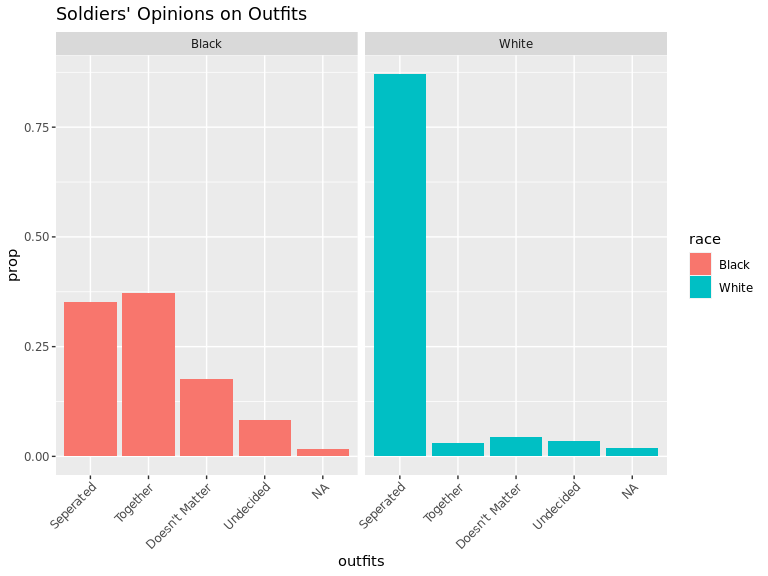
\includegraphics{consildated_overview_files/figure-latex/outfits-1.pdf}

\subsection{Deeper relationships}\label{deeper-relationships}

Of course, we are interested in seeing how these variables intearct with
one another to underdstand and reveal any deeper inticracies in the
data.

\subsubsection{Breaking down Education}\label{breaking-down-education}

When we overlay the distribution of education levels with age ranges, we
see that older white soldiers made up a larger porportion of white
soldiers with less education compared to soldiers with some high school.
As a contingent, it appears that soldiers between 21 and 24 with a high
school education make up the largest contingent of white white soldiers
when grouped by education and age.

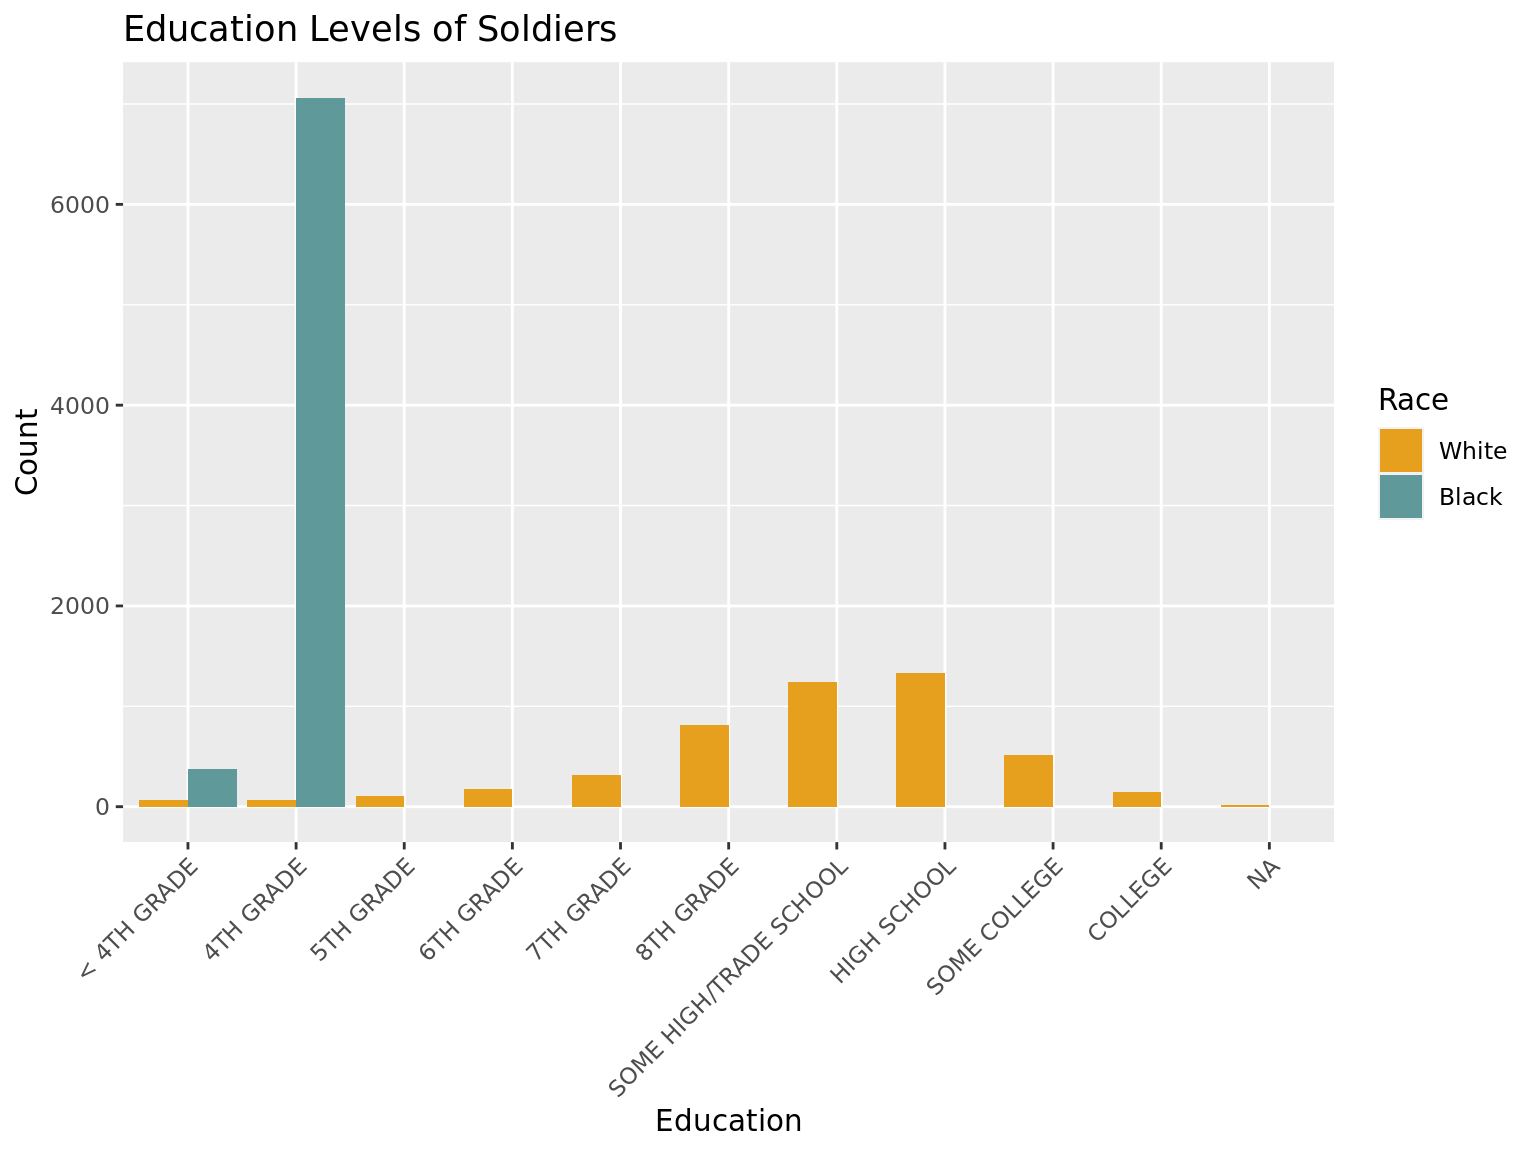
\includegraphics{consildated_overview_files/figure-latex/unnamed-chunk-3-1.pdf}
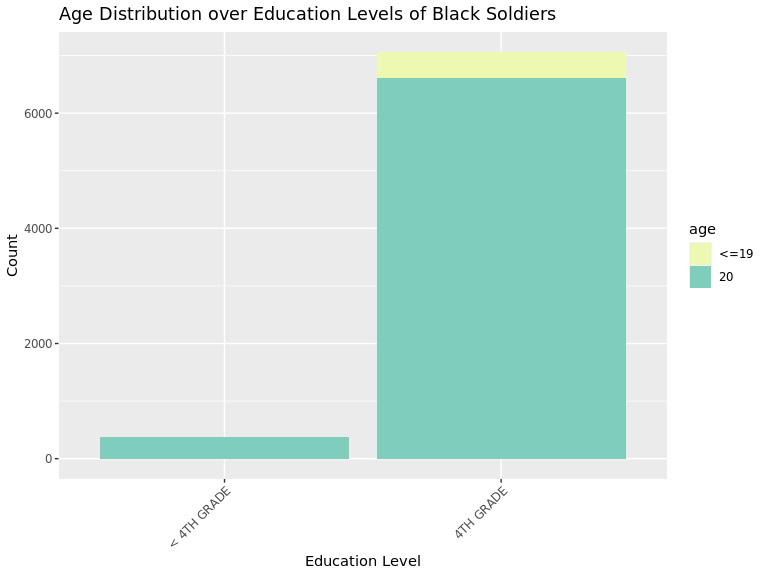
\includegraphics{consildated_overview_files/figure-latex/unnamed-chunk-3-2.pdf}
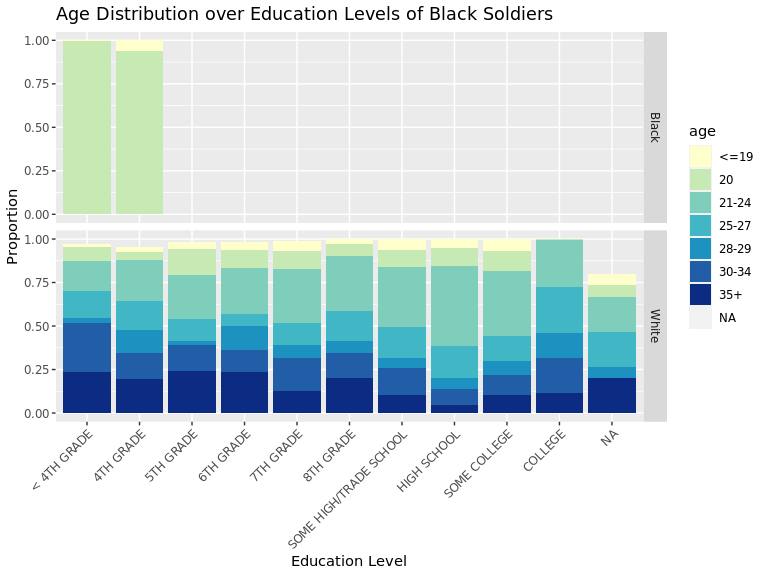
\includegraphics{consildated_overview_files/figure-latex/unnamed-chunk-3-3.pdf}

We see that larger portions of soldiers who are more educated come from
communities whihc are larger in population.

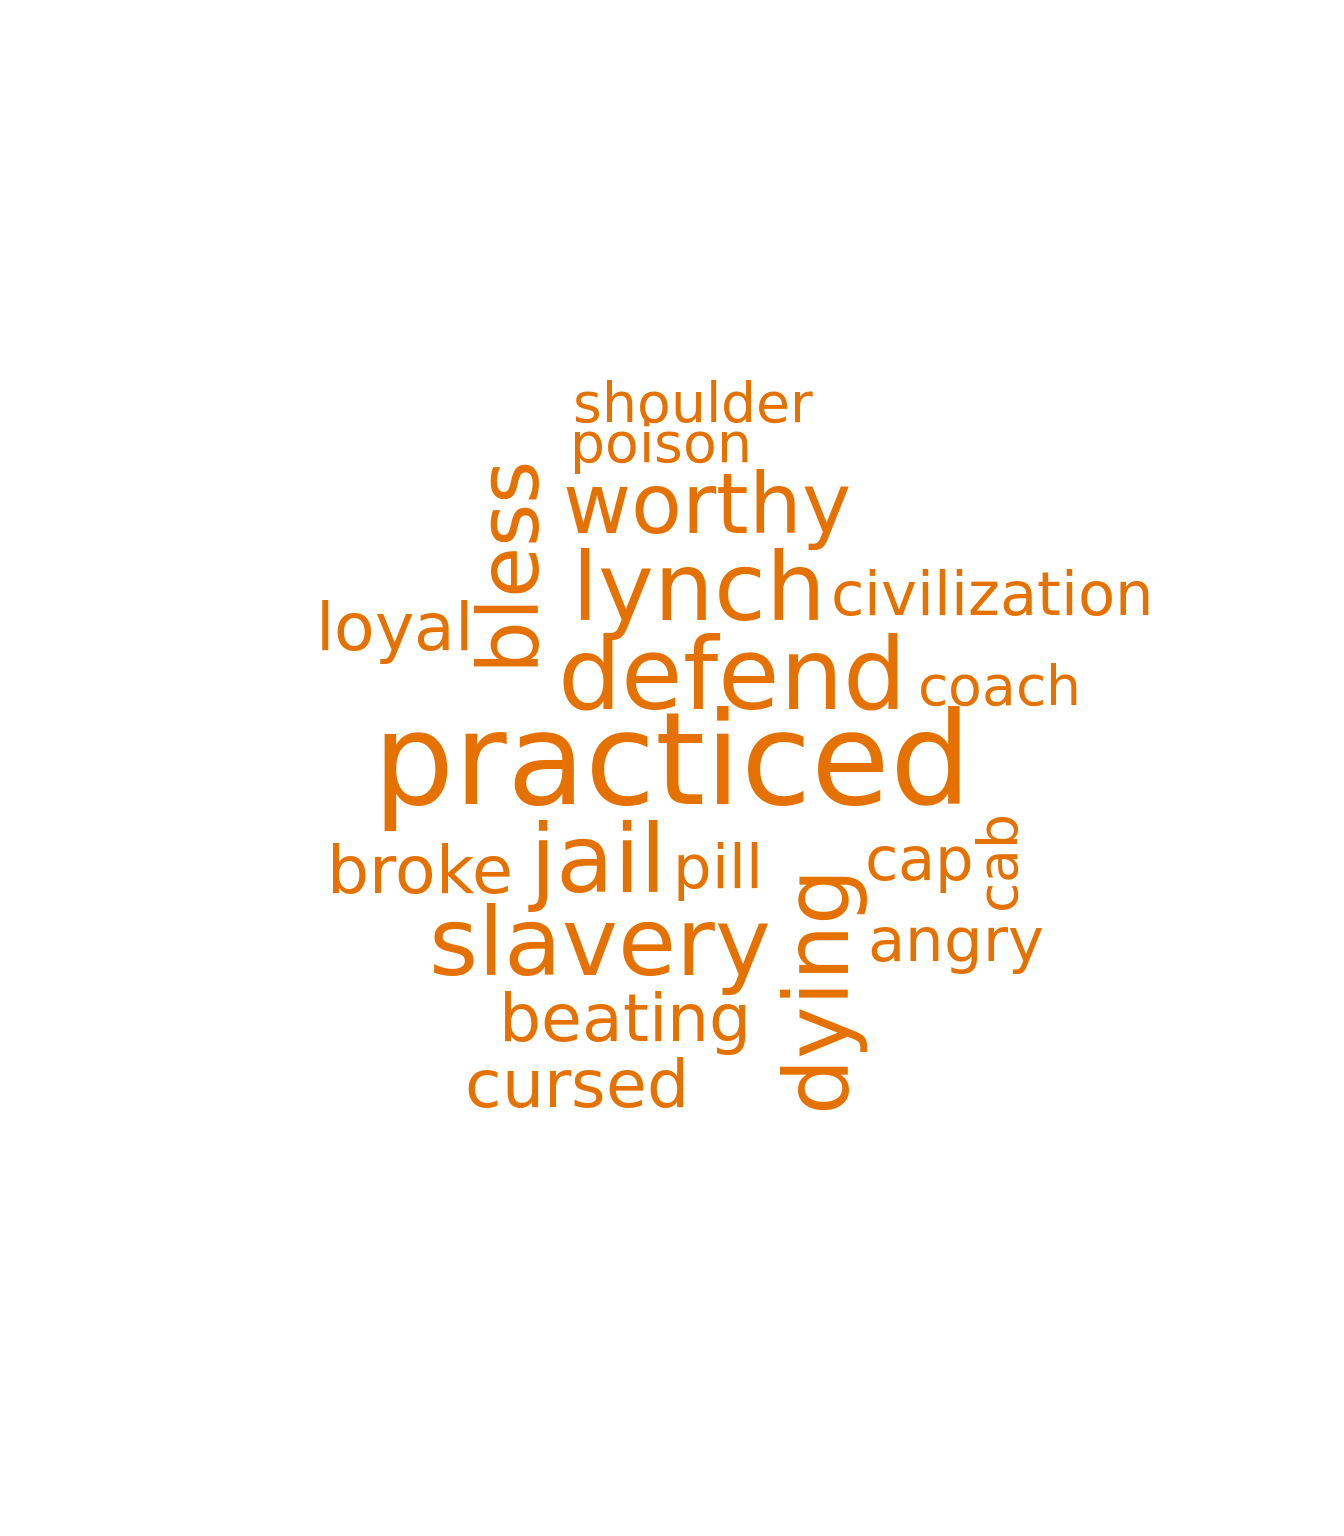
\includegraphics{consildated_overview_files/figure-latex/unnamed-chunk-5-1.pdf}
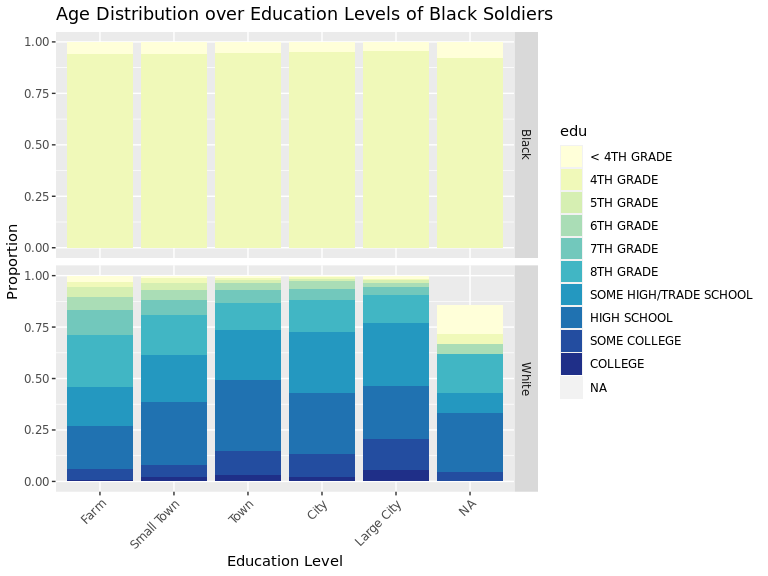
\includegraphics{consildated_overview_files/figure-latex/unnamed-chunk-5-2.pdf}

\subsubsection{Breaking Down Enlistment}\label{breaking-down-enlistment}

Due to the sample only having black soldiers no older than 20 we can't
discern if race may have an impact on how different age groups enlist.
For the most part, age makes no difference among the white soldiers in
this regard with the exception that those 19 and younger enlisted
through the draft and volunteering at similar rates. Of course, we
should keep in mind that there were not that many soldiers within this
group to begin with.
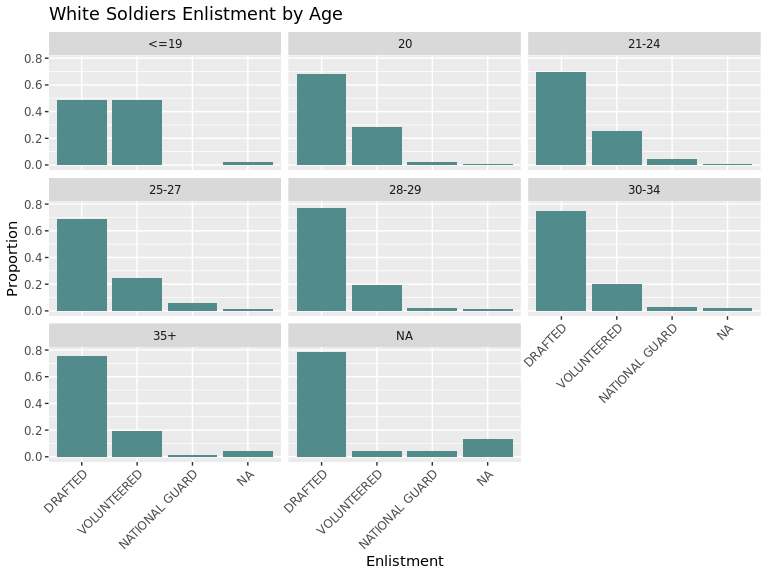
\includegraphics{consildated_overview_files/figure-latex/unnamed-chunk-6-1.pdf}
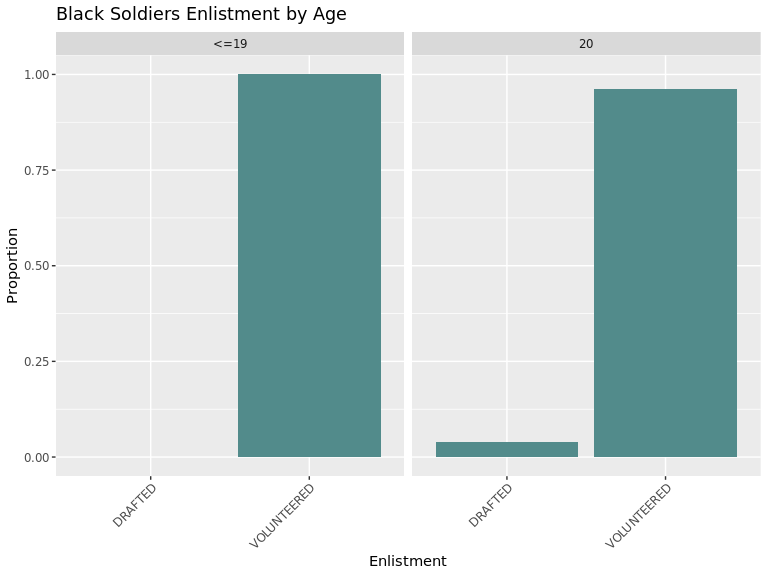
\includegraphics{consildated_overview_files/figure-latex/unnamed-chunk-6-2.pdf}
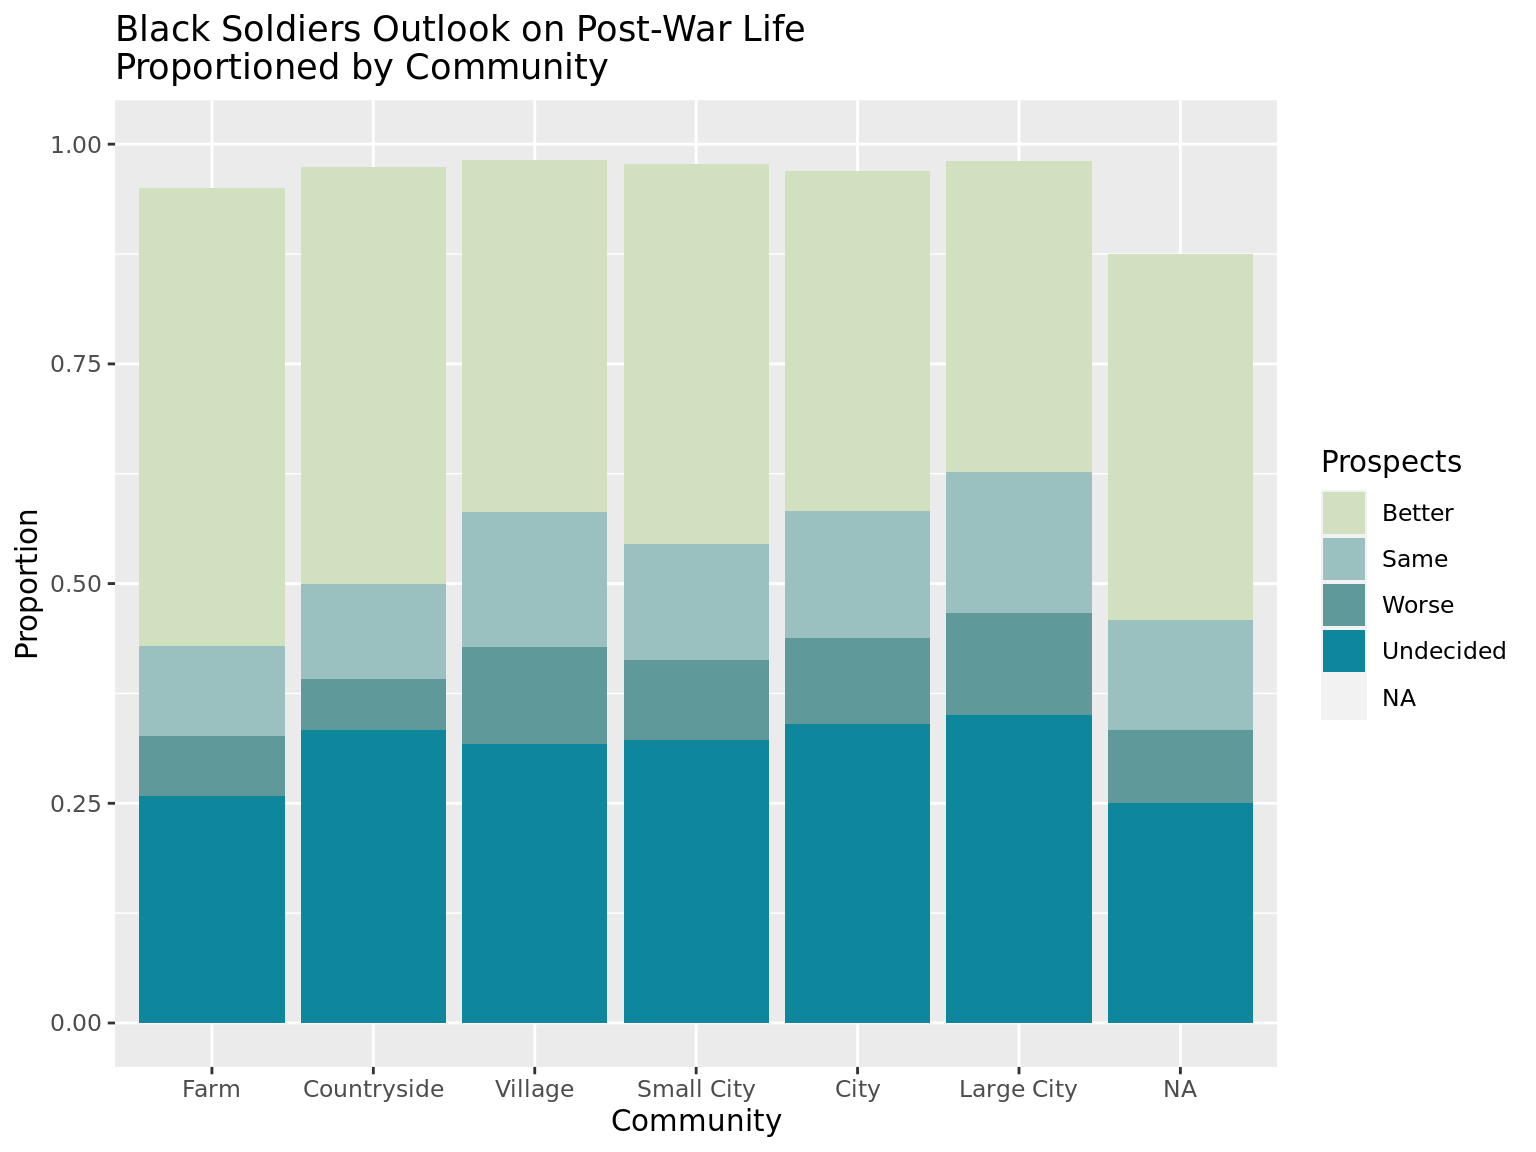
\includegraphics{consildated_overview_files/figure-latex/unnamed-chunk-6-3.pdf}

Not to interesting, white volunteered soldiers appear to be slighly
younger.
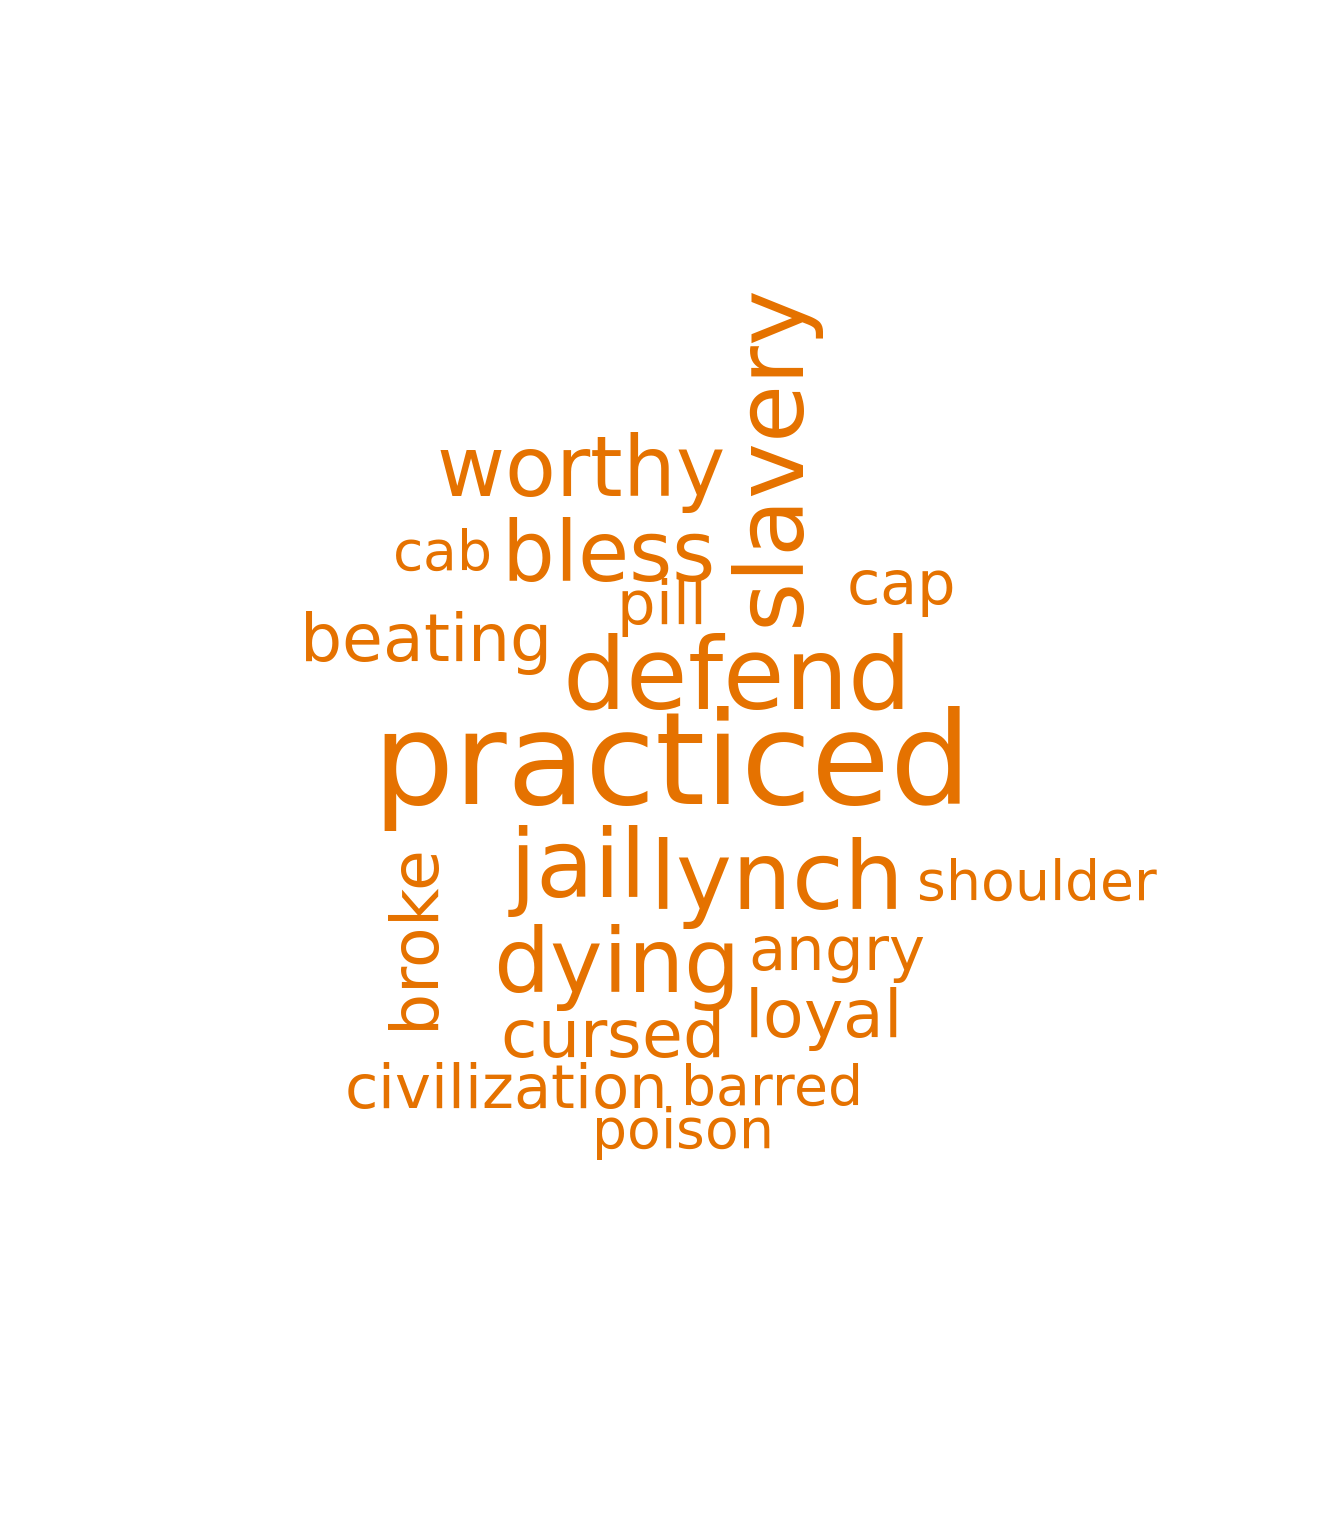
\includegraphics{consildated_overview_files/figure-latex/unnamed-chunk-7-1.pdf}
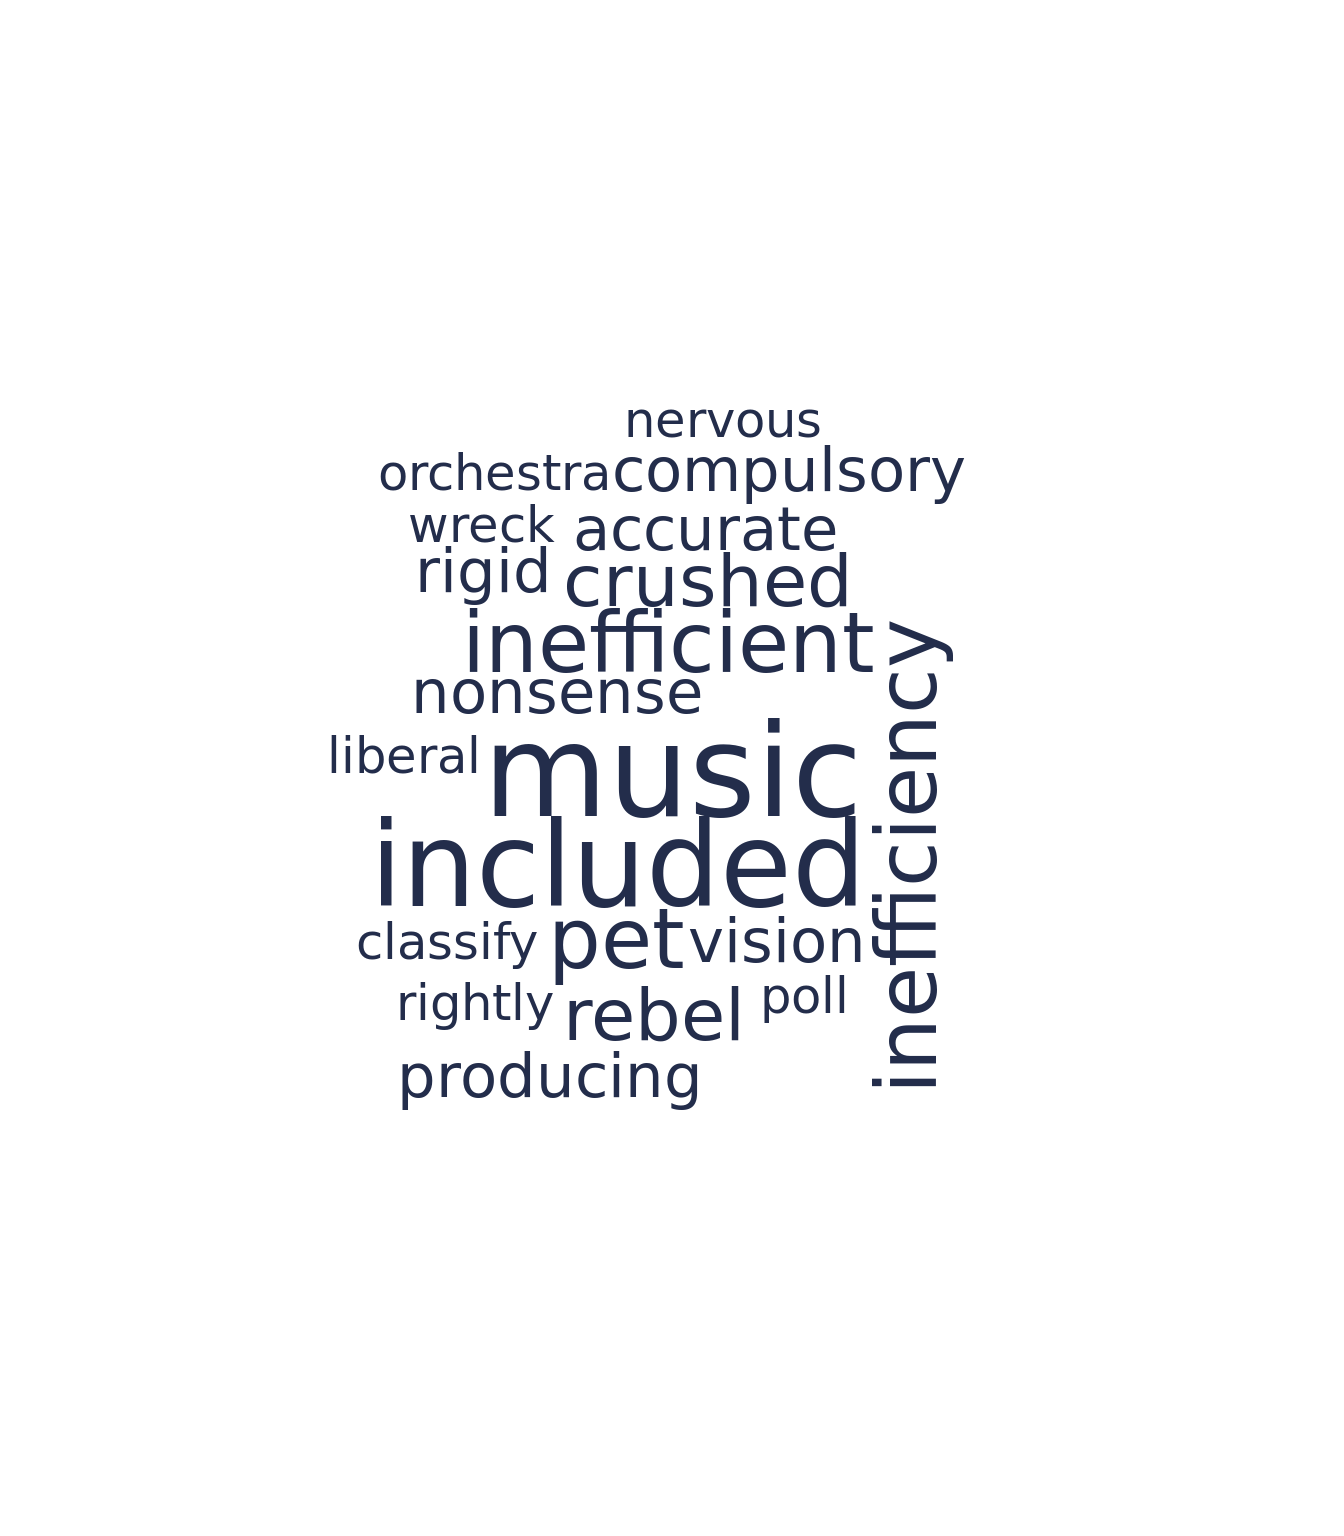
\includegraphics{consildated_overview_files/figure-latex/unnamed-chunk-7-2.pdf}

\subsubsection{Breaking Down Outfits
Opinion}\label{breaking-down-outfits-opinion}

If we look at the proportion of ages who elected for each category we
see that the proportions are relatively stable across all opinions
towards integration.

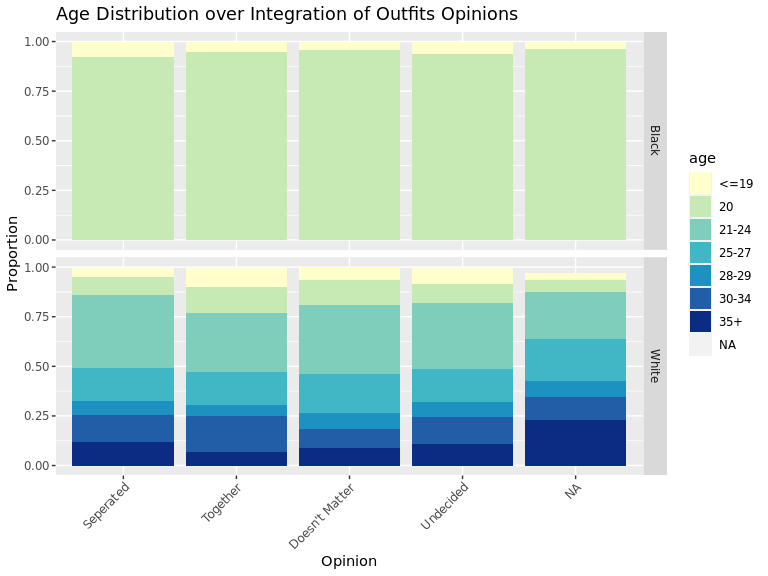
\includegraphics{consildated_overview_files/figure-latex/outfits breaking-1.pdf}
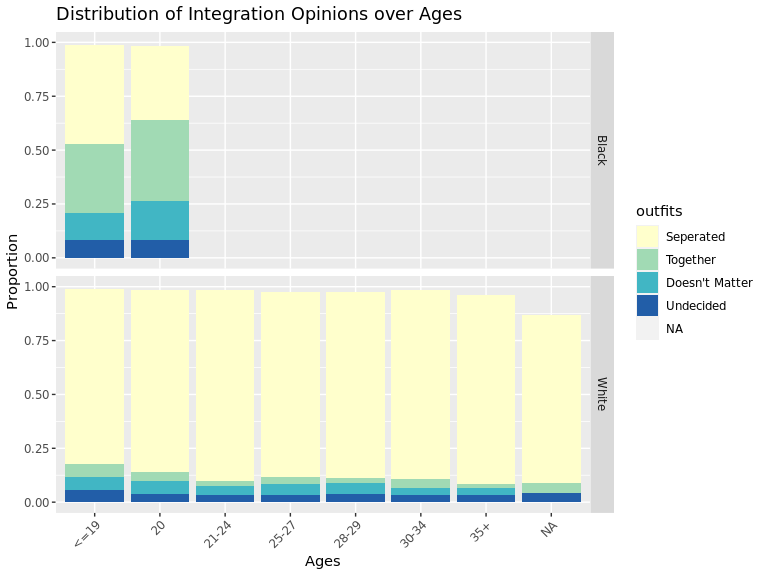
\includegraphics{consildated_overview_files/figure-latex/outfits breaking-2.pdf}

Now if we are to overlay the education distribution over the integration
opinions we see something more interesting. It appears that the white
soldiers that voted for the outfits to be together skew towards being
more educated. In fact, over 50\% of the soldiers who did vote for
integrated units have atleast finished high school. This is not the case
for any of the other responses.

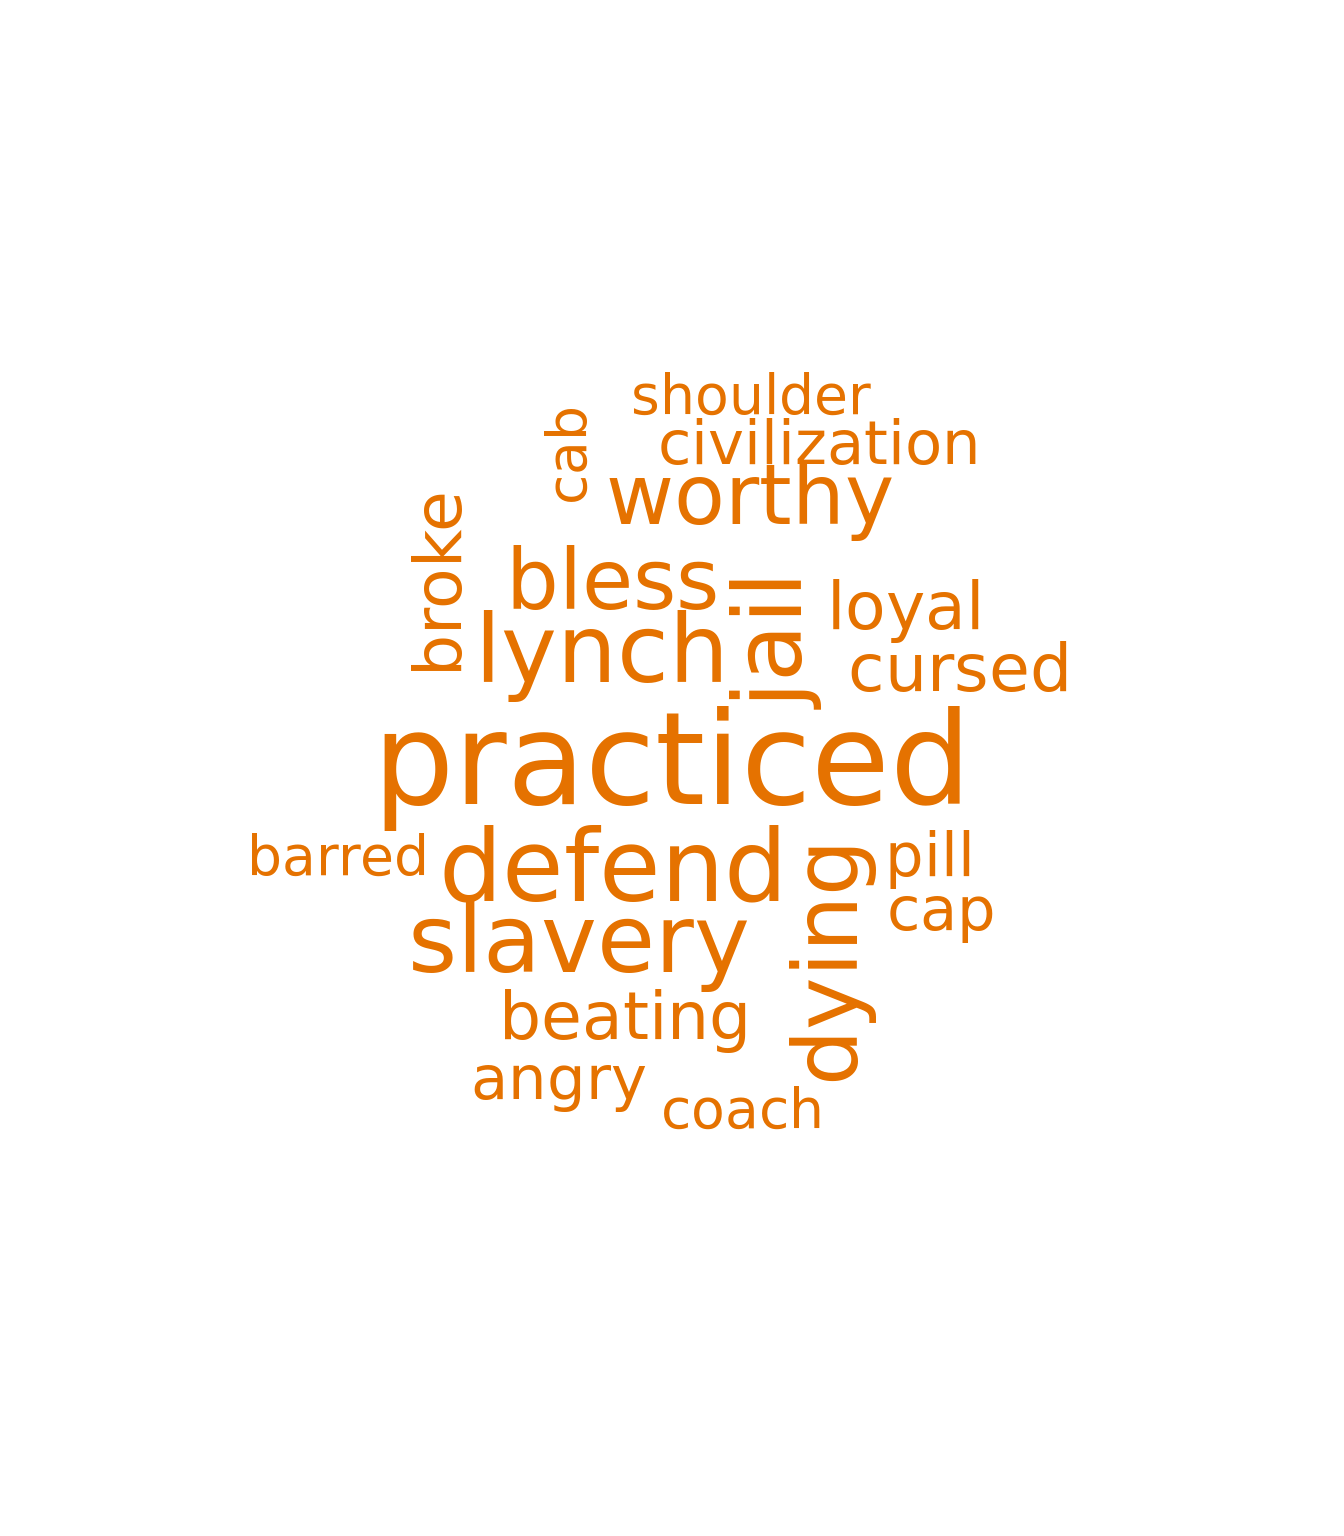
\includegraphics{consildated_overview_files/figure-latex/unnamed-chunk-8-1.pdf}

Across both races we also see that of those who choose integration a
greater portion were from large cities and soldiers who came from more
populated voted for sepration less proportionally.

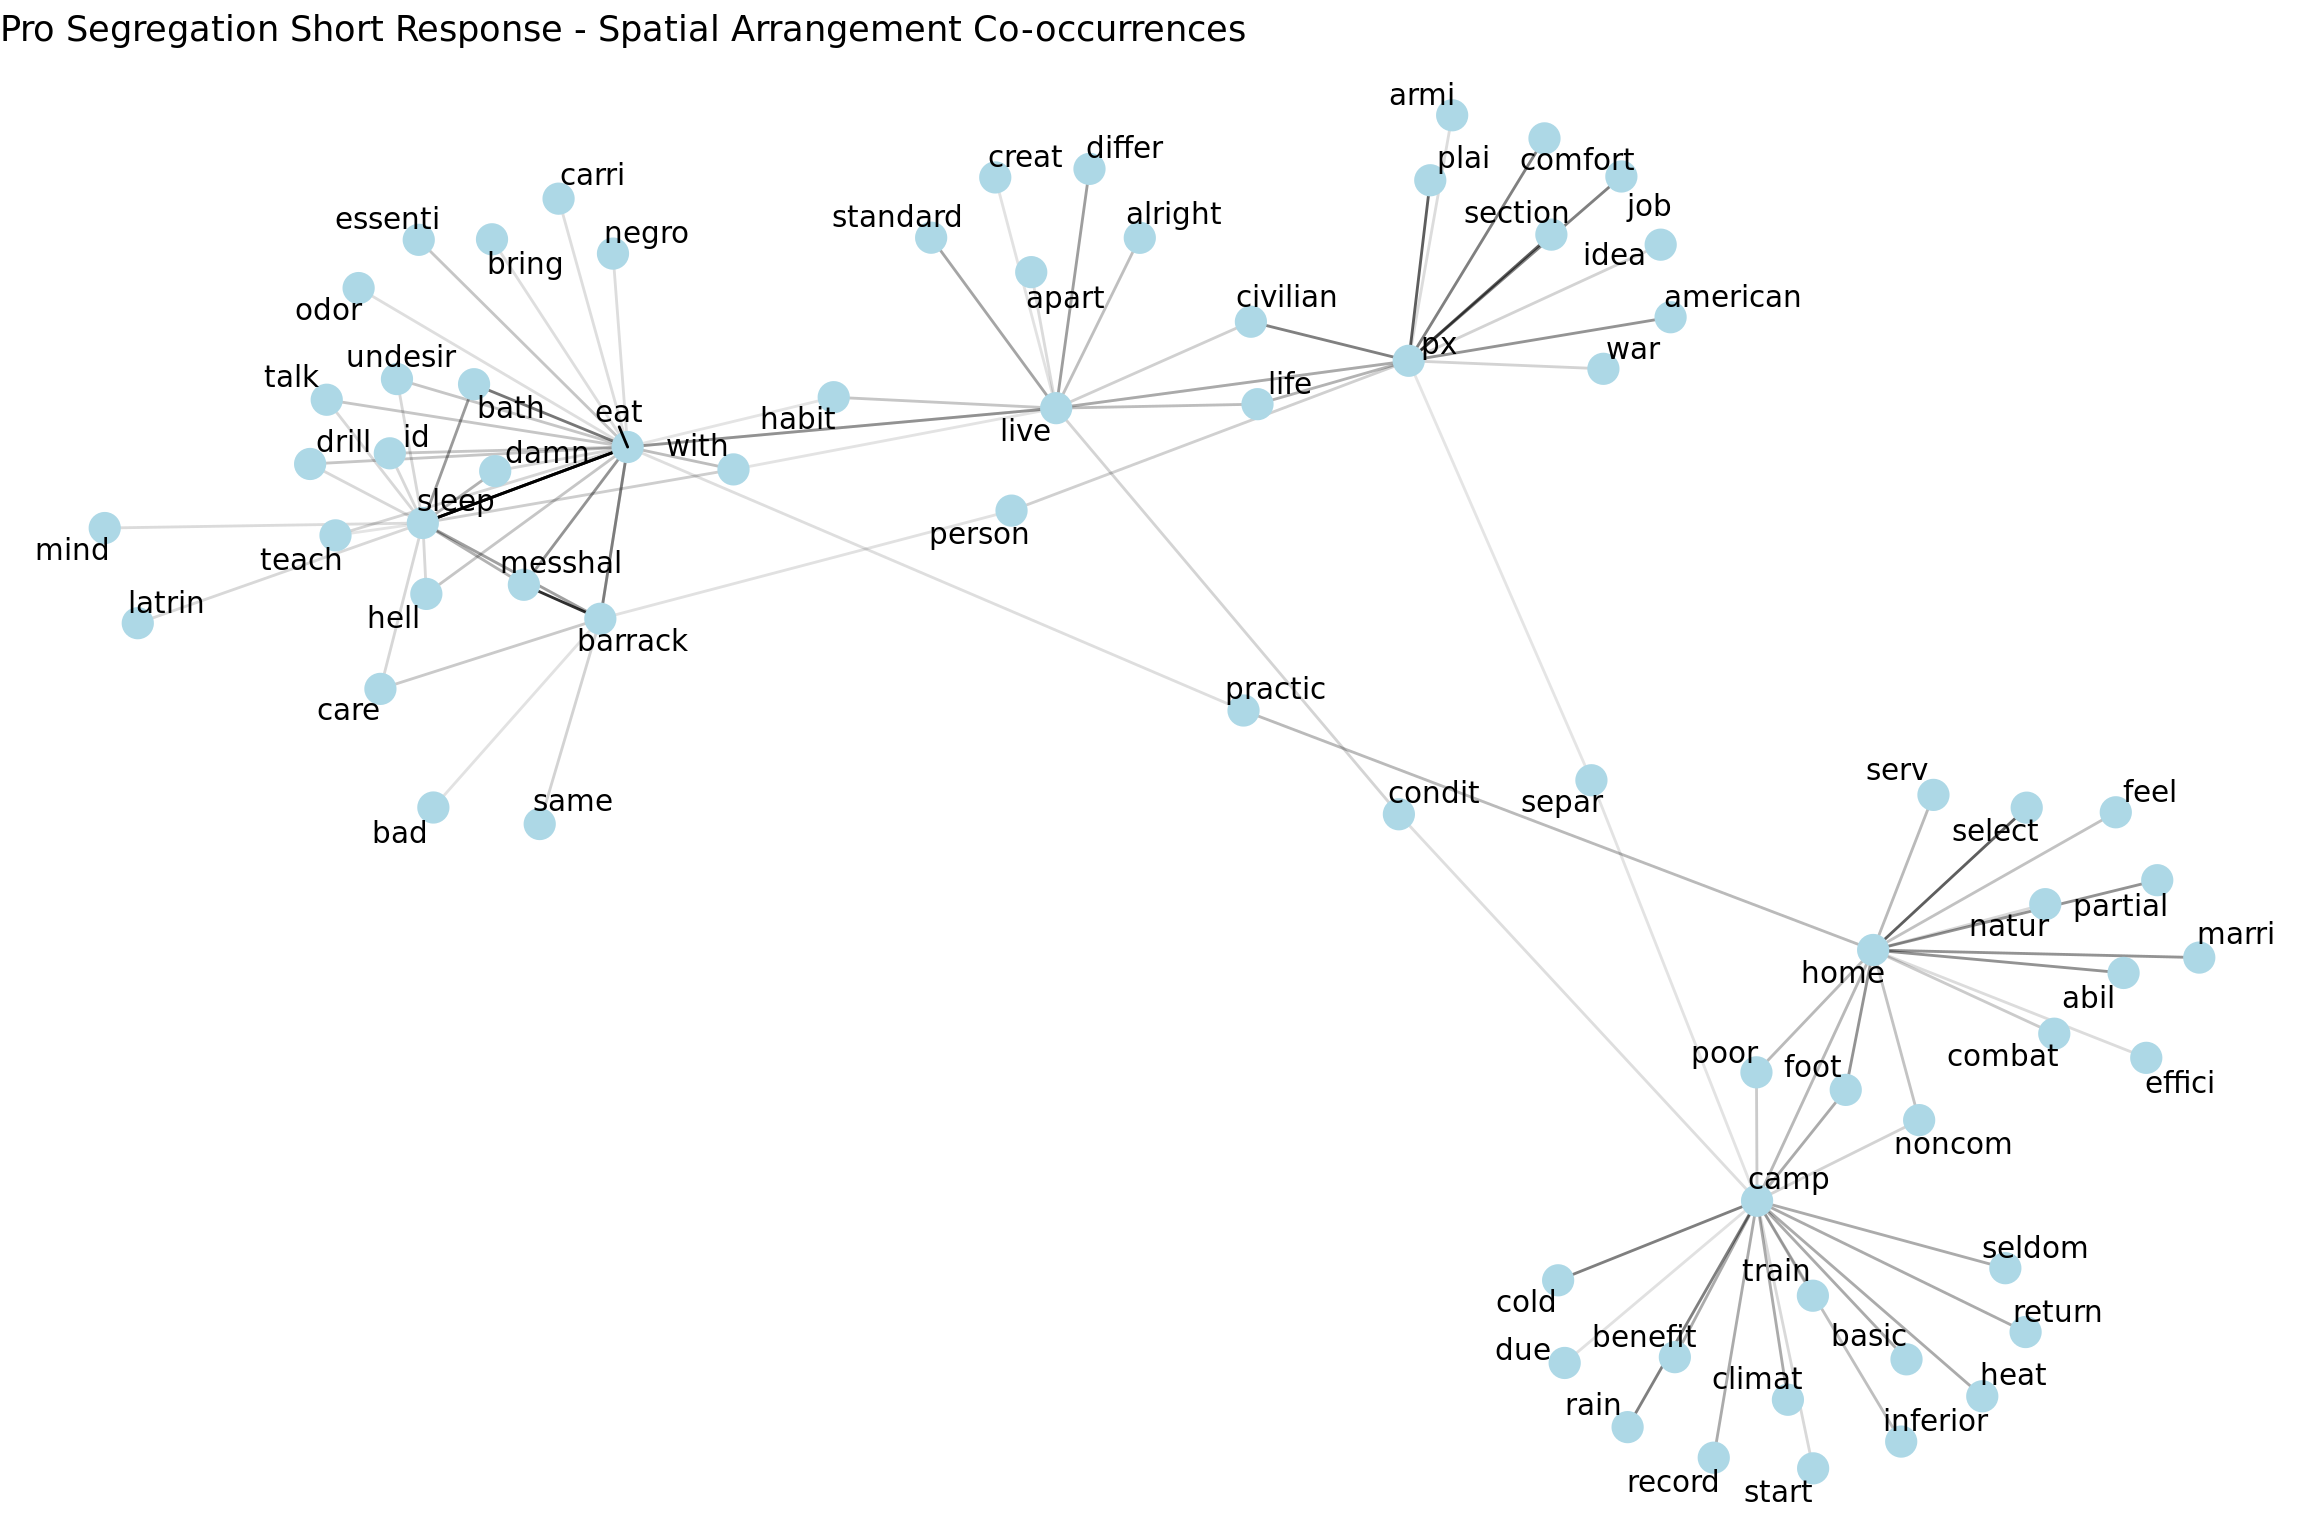
\includegraphics{consildated_overview_files/figure-latex/unnamed-chunk-9-1.pdf}
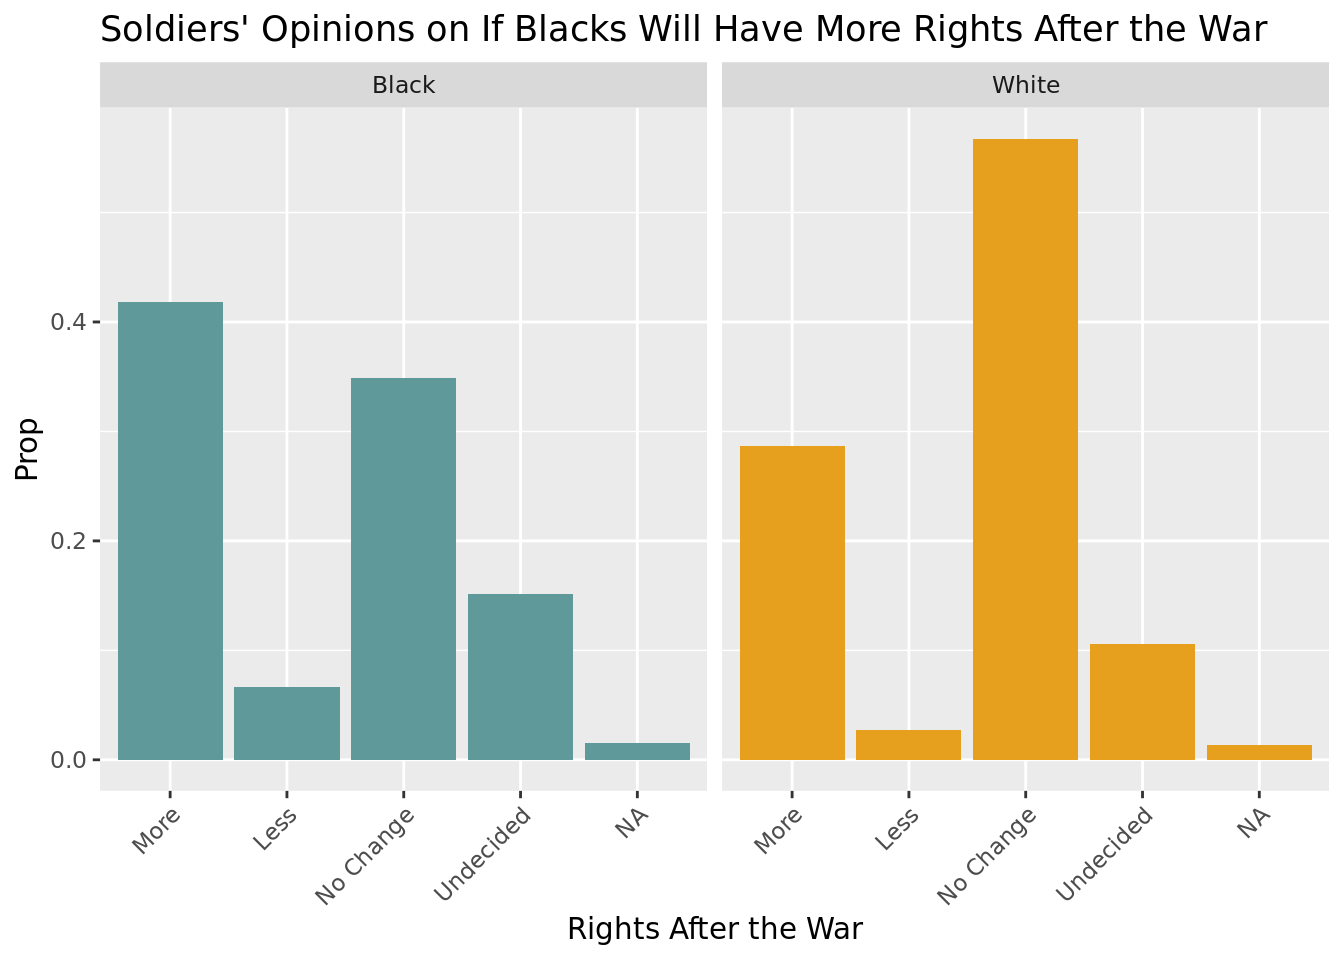
\includegraphics{consildated_overview_files/figure-latex/unnamed-chunk-9-2.pdf}
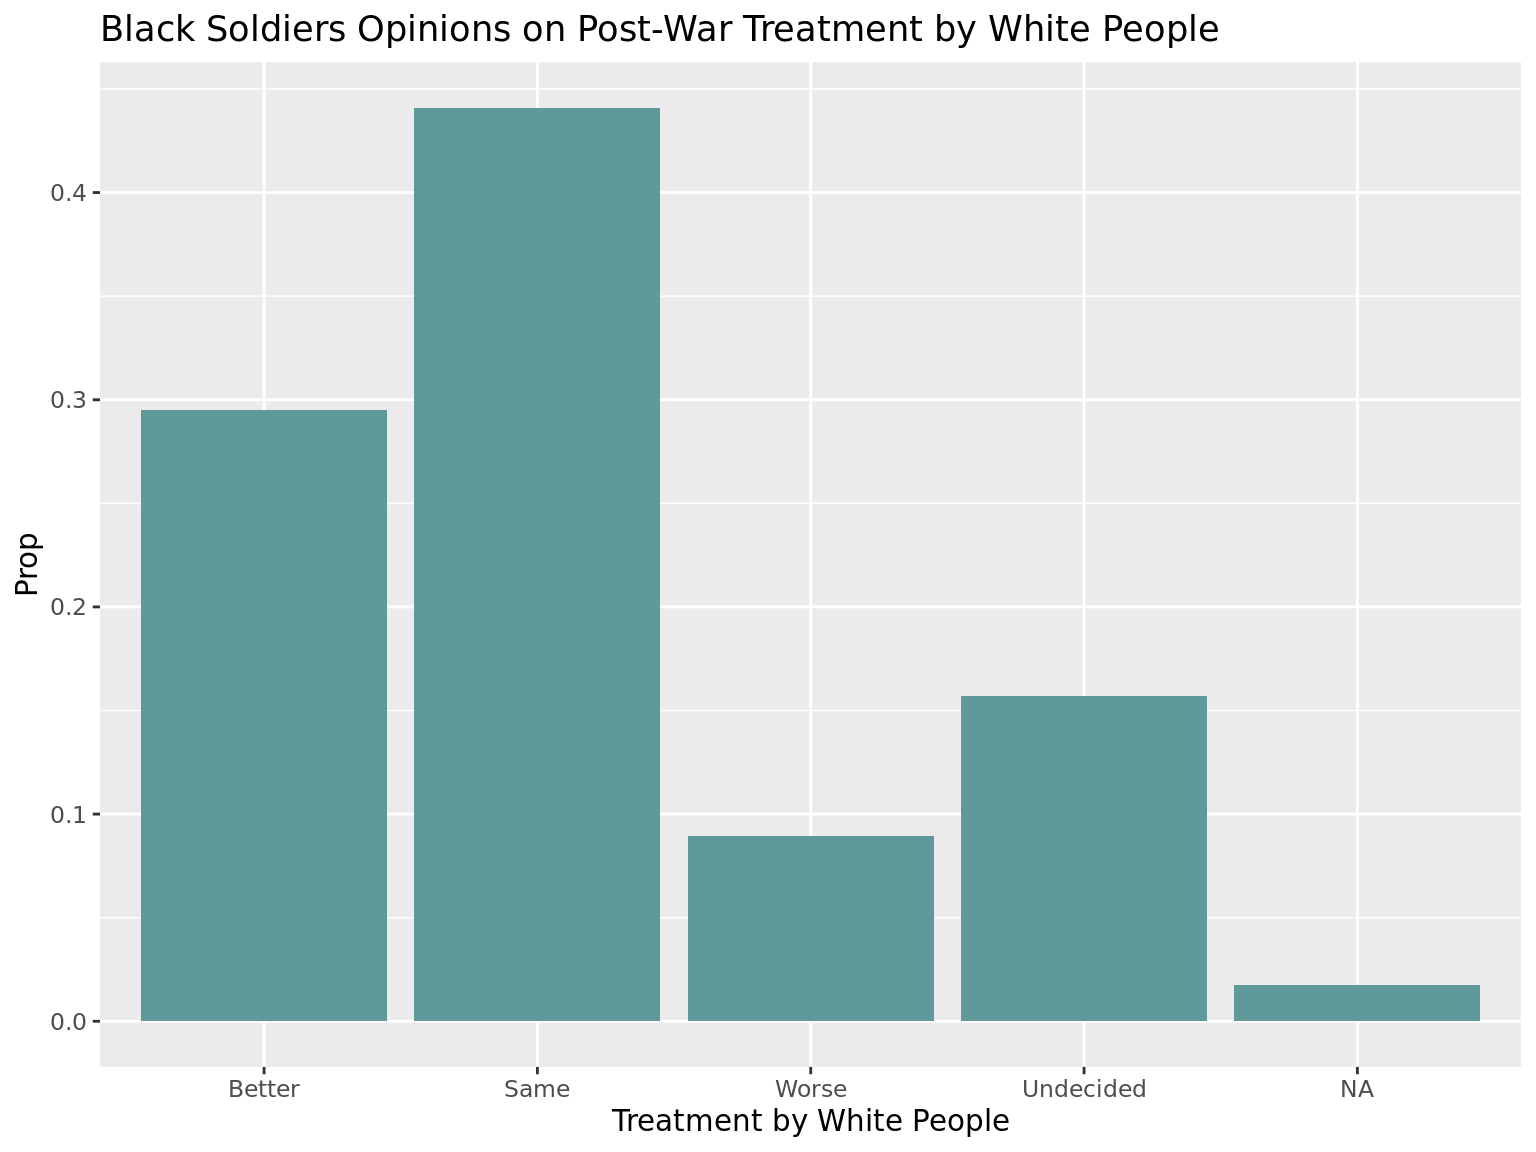
\includegraphics{consildated_overview_files/figure-latex/unnamed-chunk-9-3.pdf}

\end{document}
